%%%%%%%%%%%%%%%%%%%%%%%%
%% Sample use of the infthesis class to prepare a thesis. This can be used as 
%% a template to produce your own thesis.
%%
%% The title, abstract and so on are taken from Martin Reddy's csthesis class
%% documentation.
%%
%% MEF, October 2002
%%%%%%%%%%%%%%%%%%%%%%%%

%%%%
%% Load the class. Put any options that you want here (see the documentation
%% for the list of options). The following are samples for each type of
%% thesis:
%%
%% Note: you can also specify any of the following options:
%%  logo: put a University of Edinburgh logo onto the title page
%%  frontabs: put the abstract onto the title page
%%  deptreport: produce a title page that fits into a Computer Science
%%      departmental cover [not sure if this actually works]
%%  singlespacing, fullspacing, doublespacing: choose line spacing
%%  oneside, twoside: specify a one-sided or two-sided thesis
%%  10pt, 11pt, 12pt: choose a font size
%%  centrechapter, leftchapter, rightchapter: alignment of chapter headings
%%  sansheadings, normalheadings: headings and captions in sans-serif
%%      (default) or in the same font as the rest of the thesis
%%  [no]listsintoc: put list of figures/tables in table of contents (default:
%%      not)
%%  romanprepages, plainprepages: number the preliminary pages with Roman
%%      numerals (default) or consecutively with the rest of the thesis
%%  parskip: don't indent paragraphs, put a blank line between instead
%%  abbrevs: define a list of useful abbreviations (see documentation)
%%  draft: produce a single-spaced, double-sided thesis with narrow margins
%%
%% For a PhD thesis -- you must also specify a research institute:
%\documentclass[phd,ilcc,twoside]{infthesis}
\documentclass[mscres,icsa,logo,twoside]{infthesis}

%% For an MPhil thesis -- also needs an institute
% \documentclass[mphil,ianc]{infthesis}

%% MSc by Research, which also needs an institute
% \documentclass[mscres,irr]{infthesis}

%% Taught MSc -- specify a particular degree instead. If none is specified,
%% "MSc in Informatics" is used.
% \documentclass[msc,cogsci]{infthesis}
% \documentclass[msc]{infthesis}  % for the MSc in Informatics

%% Master of Informatics (5 year degree)


%% Logo Style: University of Edinburgh Shield
% \documentclass[minf]{infthesis}
%% Possible values for shieldtype:
%% 0: regular monochrome
%% 1: monochrome with no background lines
%% 2: reverse monochrome
%% 3: two colours: navy and red
%% 4: full colour
\shieldtype{4}

%% Undergraduate project -- specify the degree course and project type
%% separately
% \documentclass[bsc]{infthesis}
% \course{Artificial Intelligence and Psychology}
% \project{Fourth Year Project Report}

%% Put any \usepackage commands you want to use right here; the following is 
%% an example:
\usepackage{natbib}


\usepackage{float}

\usepackage{graphics}

\usepackage{graphicx}
\usepackage{subcaption}

%\usepackage{setspace}
\usepackage{ragged2e}

\usepackage[hidelinks]{hyperref}

\usepackage{amsthm}
\usepackage{amsmath,amssymb}
%\usepackage{mathrsfs}
\usepackage{mathtools}

\theoremstyle{definition}
\newtheorem{definition}{Definition}[section]
\newtheorem{prop}{Proposition}[section]

\usepackage[noend]{algpseudocode}
\usepackage{algorithm}


\newcommand{\etal}{et~al.}

\newcommand{\itercomp}{{iterative compilation}}
\newcommand{\Itercomp}{{Iterative compilation}}
\newcommand{\IterComp}{{Iterative Compilation}}

\newcommand{\flagstype}{\usefont{T1}{cmr}{m}{n}}

\usepackage{multirow}


%% Listing related stuff
\usepackage{listings}
\usepackage{courier}            %Required for pretty listings (more dense)

\usepackage[table]{xcolor}

%% EMACS colors for listing:
\usepackage{color}
\definecolor{sh_comment}{rgb}{0.65, 0.00, 0.00 } % red-ish
\definecolor{sh_keyword}{rgb}{0.37, 0.69, 0.69}  % blue-green
\definecolor{sh_string}{rgb}{0.08, 0.69, 0.08} % green

%% This manipulates the listing numbering. It decreases it by one at the point used.
\newcommand*\lstDNumber{\addtocounter{lstnumber}{-1}}

%% Change from Listing->Algorithm
%% \renewcommand\lstlistingname{Algorithm} % Fix listing caption name: Listing -> Algorithm
%% \renewcommand\lstlistlistingname{Algorithms}
%% \def\lstlistingautorefname{Alg.}

%% \renewcommand{\thelstlisting}{\thesection-\arabic{lstlisting}}
%\renewcommand{\thelstlisting}{\arabic{lstlisting}} % Fix listing numbering Algorithm 1.1 -> Algorithm 1.

%% \renewcommand{\labelenumi}{\roman{enumi}.}

\lstset{
float=[*],
language=C,                % choose the language of the code
%% basicstyle=\linespread{0.9}
%% basicstyle=\scriptsize\ttfamily,
 basicstyle={\linespread{0.97} \footnotesize\ttfamily},
 stringstyle=\color{sh_string},
 keywordstyle = \color{sh_keyword}\bfseries,
 commentstyle=\color{sh_comment}\itshape,
numbers=left,                   % where to put the line-numbers
%% numberstyle=\scriptsize,        % the size of the fonts that are used for the line-numbers
numberstyle=\scriptsize,        % the size of the fonts that are used for the line-numbers
stepnumber=1,                   % the step between two line-numbers. If it is 1 each line will be numbered
numbersep=5pt,                  % how far the line-numbers are from the code
backgroundcolor=\color{white},  % choose the background color. You must add \usepackage{color}
showspaces=false,               % show spaces adding particular underscores
showstringspaces=false,         % underline spaces within strings
showtabs=false,                 % show tabs within strings adding particular underscores
xleftmargin=2em,                % Left margin
frame=lines,                   % adds a frame around the code. none|leftline|topline|bottomline|lines|single|shadowbox
framexleftmargin=1.5em,         % Margin from frame to line numbers
framexbottommargin=0em,         % Distance from last text to frame
morekeywords={in,true,false,and,or,set,is,not},
%% prebreak=\mbox{\tiny$\searrow$},
prebreak=\space,                % Line break: insert this character at the end of the top line
%% postbreak=\mbox{{\color{blue}\scriptsize$\hookrightarrow$}}, % Line break: blue arrow at the beginning of the bottom line
postbreak=\mbox{{\color{blue}\footnotesize$\hookrightarrow$}}, % Line break: blue arrow at the beginning of the bottom line
breaklines=true,                % sets automatic line breaking
breakatwhitespace=false,        % sets if automatic breaks should only happen at whitespace
tabsize=2,                      % sets default tabsize to 2 spaces
captionpos=b,                   % sets the caption-position to top
escapeinside={\@}{\@}             % Escape sequence \@ESCAPED STUFF\@
}

\usepackage{nasm/lang}
\usepackage{nasm/style}
\usepackage{llvm/lang}


%% Information about the title, etc.
\title{Online {\IterComp}\\Guided by Work-based Profiling}
\author{Rodrigo Caetano de Oliveira Rocha}

\pdfinfo{
   /Author (Rodrigo Caetano de Oliveira Rocha)
   /Title  (Online Iterative Compilation Guided by Work-based Profiling)
   /Subject (Optimising Compilers)
   /Keywords (Iterative Compilation;Profiling;Compiler Optimisation)
}
%% If the year of submission is not the current year, uncomment this line and 
%% specify it here:
% \submityear{1785}

%% Optionally, specify the graduation month and year:
% \graduationdate{February 1786}

%% Specify the abstract here.
\abstract{%

In modern optimising compilers,  the correct choice of an optimisation sequence can have a significant impact on the performance of the final optimised program.
Each of these optimisation passes interacts with the code in complicated ways, depending on all other optimisations and the order they were applied to the code being optimised.
Because of the unpredictability of optimisation interactions and their complexity,
efficiently selecting the best optimisation sequence for a given program, or program section, remains an open problem.
A well-known compilation technique that addresses this challenge is {\itercomp}.

In this thesis, we focus on enabling {\itercomp} in \textit{online} scenarios.
We define the online scenario as having the restriction that programs execute multiple inputs and distinct inputs are executed only once.
Because of these restrictions, standard metrics for comparing optimisations, such as speedups or execution time alone, are not viable.
To address this challenge, we propose the use of a work-based performance metric for guiding {\itercomp},
where we instrument the program for measuring the amount of work it performed during its execution.
In order to reduce the profiling overhead, we also propose two relaxation algorithms which provide a trade-off between measurement accuracy and overhead.

In our experimental evaluation, the first relaxation algorithm that operates on regions of functions is able to reduce the average overhead by about 43\% over the optimal work profiling, while incurring in a dynamic measurement error of much less than 1\%.
Similarly, the second relaxation algorithm which operates on the whole program, which also makes use of profiling from previous execution, was able to reduce even further this overhead by a factor of $2.1\times$ compared to the optimal profiling, while incurring in a dynamic measurement error of less than 3\%.

Our evaluation also corroborates the use of the work-based performance metric for guiding online {\itercomp}.
Under real conditions, it was able to achieve good performance improvements when compared to the oracles, which were allowed to execute the program with the same input multiple times,
achieving an average improvement of 5.4\% and a maximum of about 20\%.
Contrary to what previous work has suggested, we have also shown that instructions per cycle (IPC) is not a good metric for guiding online {\itercomp}.
}

%% Now we start with the actual document.
\begin{document}

%% First, the preliminary pages
\begin{preliminary}

%% This creates the title page
\maketitle

%% Acknowledgements
\begin{acknowledgements}
%I would like to thank my main supervisor Hugh Leather and co-supervisors Murray Cole, Zheng Wang, and Pavlos Petoumenos
for the support offered throughout the course of this project.

This work was supported in part by the EPSRC Centre for Doctoral Training in Pervasive Parallelism, funded by the UK Engineering and Physical Sciences Research Council (grant EP/L01503X/1) and the University of Edinburgh.

I would like to thank my main supervisor Hugh Leather, as well as my co-supervisors Murray Cole, Zheng Wang, and Pavlos Petoumenos,
for the support offered throughout the course of this project.

This work was supported in part by the EPSRC Centre for Doctoral Training in Pervasive Parallelism, funded by the UK Engineering and Physical Sciences Research Council (grant EP/L01503X/1) and the University of Edinburgh.
\end{acknowledgements}

%% Next we need to have the declaration.
\standarddeclaration

%% Finally, a dedication (this is optional -- uncomment the following line if
%% you want one).
\dedication{To my parents and Isabella.}

%% Create the table of contents
\tableofcontents

%% If you want a list of figures or tables, uncomment the appropriate line(s)
\listoffigures
\listoftables

\end{preliminary}

%%%%%%%%
%% Include your chapter files here. See the sample chapter file for the basic
%% format.


\chapter{Introduction}

Modern optimising compilers have reached a high level of sophistication, providing a large number of optimisations.
Because of the unpredictability of optimisation interactions, in addition to the growing complexity of processor architectures and applications, the correct choice of optimisations and their ordering can have a significant impact on the performance of the code being optimised~\cite{pan06,fursin07,kulkarni12}.

Each of these optimisations interacts with the code in complicated ways, depending on all other optimisations and the order they were applied to the code being optimised.
Understanding the interactions of optimisations is very important in determining a good solution to the phase-ordering problem~\cite{touati06,kulkarni12}.
Because of all those dependencies and interactions, although most compiler optimisations yield significant improvements in many programs, the potential for performance degradation in certain program patterns is known to compiler writers and many users~\cite{pan06,zhou12,kulkarni12}.
%Traditional compilers typically apply the same set of optimisation in a fixed order to all functions in a program, without regard the code being optimised.

Efficiently selecting the best combination of compiler optimisations for a given program or program section remains an open problem.
Compiler writers typically use a combination of experience and insight to construct the default sequences of prearranged optimisations found in compilers.
However, these default pre-arranged set of optimisations do not include all possible optimisations and they are always applied in the same pre-defined fixed order, without regard the code being optimised~\cite{pan06,cavazos07,zhou12,kulkarni12}.
%in hopes that a programmer will know which combination of optimisations will benefit their code~\cite{pan06,cavazos07,zhou12,kulkarni12}.

A well known compilation technique that addresses this challenge is {\itercomp}.
{\Itercomp} has the ability to adapt to new platforms, program and workload while still having a systematic and simple optimisation process.
It works by repeatedly evaluating a large number of compiler optimisations until the best combination is found for a particular program~\cite{fursin07,chen10}.
The main challenge concerning {\itercomp} is the need for efficiently exploring such a large optimisation space~\cite{fursin07,cavazos07,zhou12}.

Until recently, most of existing work  had been focusing on finding the best optimisation through repeated runs using a single input.
Although they demonstrate the potential of {\itercomp}, in real scenarios the user rarely executes the same input dataset multiple times~\cite{bodin98,kisuki99,stephenson03,kulkarni04,agakov06}.
Applying {\itercomp} in light of a single input may not result in good performance when executing the optimised code with different inputs.

Most of real world applications are complex enough so that a single input case does not capture the whole range of possible scenarios and program behaviour~\cite{haneda06,fursin07,chen10,chen12a}.
Because programs can exhibit behaviours that differ greatly depending on the input,
%This is something that is well known when writing test cases for correctness.
%We can extend the same argument when optimising the code for performance.
using a single input for {\itercomp} can produce poor performance when executed with different inputs.

Recent work have been studying the impact of using multiple input datasets
for performing {\itercomp}.
This previous work suggests that optimising based on a representative range of input datasets allows for selecting a robust compiler optimisation that produces good performance in real scenarios where the input is expected to change constantly~\cite{haneda06,fursin07,chen10,chen12a,chen12b,fang15,mpeis16}.
Their results show that a limited number of input datasets may be sufficient to obtain a well optimised program for a wider range of different inputs~\cite{haneda06,fursin07,chen10,chen12a}.

Finding such a robust combination of compiler optimisations by means of {\itercomp} across a large range of inputs may be very time consuming.
In order to speed up this process we intend to reduce the number of actual executions during the exploration of the optimisation space without much degradation of the final selected optimisation.

\begin{figure}[htb]
    \centering
    \includegraphics[width=\linewidth]{figs/diagram}
    \caption{Overview of the execution engine for applying {\itercomp}.}
    \label{fig:diagram}
\end{figure}

In this paper, our main goal is to enable {\itercomp} in \textit{online} scenarios with the restriction of executing distinct inputs only once, while targeting optimal performance across different inputs.
This online aspect is usually found in mobile and data centre platforms~\cite{chen12b,fang15,mpeis16}, where the goal is to optimise programs based on the workload of a particular user (or group of users) between executions.

Measuring just execution time, for example, is useful only if the amount of work is constant between executions with different inputs.
For this reason, we propose the use of a work-based metric in order to compare the performance of different optimisations across multiple executions of the program with distinct inputs.

Because of the restriction of not repeating inputs, we instrument the program for measuring the amount of work it performed during its execution.
Having a low overhead instrumentation is essential in this online scenario for two main reasons:
$(i)$ the user is directly affected by large overheads;
$(ii)$ a highly intrusive instrumentation can havea significant impact on the effect of the optimisations.

Our main contributions are the following:
\begin{itemize}
\item The use of a work-based performance metric in order to enable \textit{online} {\itercomp} by comparing different combination of compiler optimisations even when executed with distinct inputs.
\item We propose a relaxed instrumentation for low overhead profiling, with a controlled trade-off between accuracy and overhead.
\end{itemize}


\chapter{Background}

\section{Early Work in {\IterComp}}

\textbf{Original work in {\IterComp}: single input and offline}

\section{Program Profiling}

\textbf{Basic background about profiling in general}

\section{LLVM Compiler Infrastructure}

LLVM is a compiler framework that implements the classical \textit{three-phase compiler} infrastructure, which consists of a frontend, an optimiser, and a backend.

The frontend is responsible for parsing, validating and diagnosing errors in the source code.
This parsed source code is then translated into LLVM Intermediate Representation (IR).
The optimiser is responsible for doing a broad variety of transformations to try to improve the code's running time, such as eliminating redundant computations, and is usually more or less independent of language and target.
%The front end parses source code, checking it for errors, and builds a language-specific Abstract Syntax Tree (AST) to represent the input code. The AST is optionally converted to a new representation for optimization, and the optimizer and back end are run on the code.
%The optimizer is responsible for doing a broad variety of transformations to try to improve the code's running time, such as eliminating redundant computations, and is usually more or less independent of language and target.
The backend (also known as the code generator) then maps the code onto the target instruction set. In addition to making correct code, it is responsible for generating good code that takes advantage of unusual features of the supported architecture. Common parts of a compiler back end include instruction selection, register allocation, and instruction scheduling.
%This IR is optionally fed through a series of analysis and optimization passes which improve the code, then is sent into a code generator to produce native machine code, as shown in Figure 11.3.
%This is a very straightforward implementation of the three-phase design, but this simple description glosses over some of the power and flexibility that the LLVM architecture derives from LLVM IR.

%The most important aspect of its design is the LLVM Intermediate Representation (IR), which is the form it uses to represent code in the compiler.
%LLVM IR is designed to host mid-level analyses and transformations that you find in the optimizer section of a compiler.
%It was designed with many specific goals in mind, including supporting lightweight runtime optimizations, interprocedural optimizations, whole program analysis, and aggressive restructuring transformations, etc.
LLVM IR is a low-level RISC-like virtual instruction set.
Like a real RISC instruction set, it supports linear sequences of simple instructions like add, subtract, compare, and branch.

It differs from other intermediate representations (e.g. GCC's GENERICS or the most recent GCC's GIMPLE) as it is defined as a first class language with well-defined semantics.

The LLVM code representation describes a program using
an abstract RISC-like instruction set but with key higherlevel
information for effective analysis. This includes type
information, explicit control flow graphs, and an explicit
dataflow representation (using an infinite, typed register set
in Static Single Assignment form [15]). There are several
novel features in the LLVM code representation: (a) A lowlevel,
language-independent type system that can be used to
implement data types and operations from high-level languages,
exposing their implementation behavior to all stages
of optimization. This type system includes the type information
used by sophisticated (but language-independent)
techniques, such as algorithms for pointer analysis, dependence
analysis, and data transformations. (b) Instructions
for performing type conversions and low-level address arithmetic
while preserving type information. (c) Two low-level
exception-handling instructions for implementing languagespecific
exception semantics, while explicitly exposing exceptional
control flow to the compiler.


These instructions are in three address form, which means that they take some number of inputs and produce a result in a different register.5 LLVM IR supports labels and generally looks like a weird form of assembly language.

Unlike most RISC instruction sets, LLVM is strongly typed with a simple type system (e.g., i32 is a 32-bit integer, i32** is a pointer to pointer to 32-bit integer) and some details of the machine are abstracted away. For example, the calling convention is abstracted through call and ret instructions and explicit arguments. Another significant difference from machine code is that the LLVM IR doesn't use a fixed set of named registers, it uses an infinite set of temporaries named with a % character.

Beyond being implemented as a language, LLVM IR is actually defined in three isomorphic forms: the textual format above, an in-memory data structure inspected and modified by optimizations themselves, and an efficient and dense on-disk binary "bitcode" format. The LLVM Project also provides tools to convert the on-disk format from text to binary: llvm-as assembles the textual .ll file into a .bc file containing the bitcode goop and llvm-dis turns a .bc file into a .ll file.

***LLVM IR is a Complete Code Representation***
In particular, LLVM IR is both well specified and the only interface to the optimizer. This property means that all you need to know to write a front end for LLVM is what LLVM IR is, how it works, and the invariants it expects. Since LLVM IR has a first-class textual form, it is both possible and reasonable to build a front end that outputs LLVM IR as text, then uses Unix pipes to send it through the optimizer sequence and code generator of your choice.

It might be surprising, but this is actually a pretty novel property to LLVM and one of the major reasons for its success in a broad range of different applications. Even the widely successful and relatively well-architected GCC compiler does not have this property: its GIMPLE mid-level representation is not a self-contained representation. As a simple example, when the GCC code generator goes to emit DWARF debug information, it reaches back and walks the source level "tree" form. GIMPLE itself uses a "tuple" representation for the operations in the code, but (at least as of GCC 4.5) still represents operands as references back to the source level tree form.

The implications of this are that front-end authors need to know and produce GCC's tree data structures as well as GIMPLE to write a GCC front end. The GCC back end has similar problems, so they also need to know bits and pieces of how the RTL back end works as well. Finally, GCC doesn't have a way to dump out "everything representing my code", or a way to read and write GIMPLE (and the related data structures that form the representation of the code) in text form. The result is that it is relatively hard to experiment with GCC, and therefore it has relatively few front ends.


\textbf{IR, what is a Basic Block, SSA Form}

\chapter{Related Work}

\section{{\IterComp}}

\textbf{Specific work in {\IterComp} about multiple inputs and online scenarios}

\cite{chen10,chen12a} evaluate the effectiveness of iterative compilations across a large number of input test cases.
Their main motivation is to answer the question:
\textit{How data input dependent is {\itercomp}?}
Their results show that it is possible to find a combination of compiler optimisations that achieves at least 86\% of the maximum speedup across all input test cases.
These optimal combinations are program-specific and yield average speedups up to 3.75$\times$ over the highest optimisation level of compilers.

When optimising a program, the main method for {\itercomp} used by \cite{chen10,chen12a} evaluates each combination of compiler optimisations across all the available inputs, i.e., if $N$ is the number of input test cases and $M$ is the total number of combinations of compiler optimisations, they perform a total of $O(NM)$ runs of the program being optimised.
Furthermore, they use a pre-defined set of only 300 different combinations of compiler optimisations, which represents a very small sample of the optimisation search space for most modern compilers, e.g.
LLVM has 56 distinct optimisation passes and GCC has about 47 high-level (SSA form) optimisation passes and about 25 low-level (RTL) optimisation passes, which in both cases result in much more than $2^{50}$ distinct combinations of compiler optimisations, without considering repetition.

Recent work~\citep{chen12b,fang15} have applied the same idea of performing input-dependent {\itercomp} to distributed applications on data centres.
In summary, each worker receives a subset of the input dataset, called the evaluation dataset, to perform an \textit{online} {\itercomp} of the code being executed.
Each worker performs the same the method for {\itercomp} used by \cite{chen10,chen12a}, i.e., they evaluate each combination of compiler optimisations across all the evaluation dataset.
However, because the optimisation is performed online, they usually consider a small evaluation dataset and a small number of compiler optimisations.

\cite{fursin07} addressed the problem of comparing the effect of two optimisations on two distinct inputs. For that purpose, they proposed to use instruction per cycle (IPC) as the metric for performing such comparison.
Their result show that using IPC seems promising as a robust metric for {\itercomp} across large input datasets.
However, some specific optimisation techniques may affect the use of IPC as a robust metric, and specially IPC has been shown to provide poor performance estimation for multi-threaded programs~\citep{alameldeen06,eyerman08}.
In particular, IPC can give a skewed performance measure if threads spend time in \textit{spin-lock loops} or other synchronisation mechanisms. 
Some existing work on performance assessment suggest that total execution time should be used for measuring performance of multi-threaded programs~\citep{alameldeen06,eyerman08}.
\cite{alameldeen06} in particular suggest that a simple work-related metric should be used if the unit of work is representative enough.
Work-related metrics have already been largely used for measuring performance of throughput-oriented applications, for other applications, however, choosing an appropriate unit of work can be more challenging~\citep{alameldeen06}.

\section{Work and Input Size Metrics}

\textbf{Talk about work-based metrics}

Previous work have proposed profiling-based mechanism to estimate input sizes~\citep{zaparanuks12,coppa14}.
\cite{coppa14} in particular propose the concept of \textit{read memory size} for automatically estimating the size of the input passed to a routine, where \textit{read memory size} represents the number of distinct memory cells first accessed by a read operation.
In other words, the \textit{read memory size} metric measures the size of the useful portion of the input's memory footprint.
However, because we are interested in the amount of computational work performed in respect of a given input, the memory footprint of the input may not always have a direct correspondence to  the amount of computational work.

\cite{goldsmith07} use \textit{block frequency} as the measure for performance for empirically describing the asymptotic behaviour of programs, which is known as empirical computational complexity.
Block frequency is a relative metric that represents the number of times a basic block executes~\citep{ball94,ball96}.
They argue in favour of block frequency due to its portability, repeatability and exactness, since it does not suffer from timer resolution problems or non-deterministic noises.
Block frequency also has the advantage of being efficiently profiled by means of automatic code instrumentation~\citep{knuth73,ball94}.

However, in the context of comparing different optimisations, although block frequency would be able to capture aspects of optimisations that simplify the control-flow graph (CFG), measuring work at the basic block resolution would not capture effects of optimisations at the instruction level.
Because of that, we extend the idea of using basic block frequency to measure computational work by also considering the computational cost of each basic block.
The computational cost of a basic block is given by weighting the instructions that it contains.

\section{Optimal Instrumentation} \label{subsec:optimalInstrumentation}

In order to profile  block frequency, the program can be instrumented with counters that determine how many times each basic block in a program executes.
A naive instrumentation would consist basically of having a counter for each basic block which is incremented every time the basic block is reached.
Although the naive instrumentation was commonly used in practice~\citep{knuth71}, it is a very invasive instrumentation that imposes an unnecessarily high overhead in the instrumented program.
An optimal instrumentation based on the principle of \textit{conservation of flow} (\textit{Kirchhoff's first law}\footnote{Gustav Kirchhoff defined two equalities about electric circuits, known as Kirchhoff's circuit laws. The first one is about current and and the second about potential difference.}) have been originally proposed by \cite{nahapetian73} and \cite{knuth73}.
While \cite{knuth73} proposed an optimal solution for basic block profiling with \textit{vertex counters}, \cite{ball94} showed that an optimal basic block profiling with \textit{edge counters} provides the best instrumentation for block frequency profiling.
Further overhead reduction of the optimal instrumentation was later proposed by placing the counters in edges that are less likely to be executed~\cite{forman81,ball94}.

\begin{definition}[Kirchhoff's first law]
The amount of flow into a vertex equals the amount of output flow, i.e. the sum of the incoming edges of a vertex equals the sum of outgoing edges of the same vertex.
\end{definition}

The optimal instrumentation places probes in edges as the basic block frequency can be derived by summing either the flow of the incoming or outgoing edges.
However, it uses the Kirchhoff's first law in order to place probes in subset of the edges that allows to later infer the flow of all edges.
Previous work have shown that a set of edges represents the minimum number of probes for profiling block frequency if and only if the complementary set of edges forms a spanning tree~\citep{nahapetian73,ball94}.
In other words, after determining a spanning tree of the CFG, probes need to be placed only in the edges from the complement of a spanning tree, usually called \textit{cotree}.
Because the edge frequencies satisfy Kirchhoff's first law, each edge flow can be uniquely determined as an algebraic sum of the known edge flows from the cotree~\citep{nahapetian73,ball94}.

\begin{lstlisting}[caption={A data-flow analysis for populating all edge flows based on the probed edges.}, label={lst:populateEdgeFlows}, float]
// Inputs: CFG with the known edges flows from the cotree
// Output: Updated CFG with all edge flows
populateEdgeFlows(G) {
  changed = true
  while changed:
    changed = false
    for B in G.vertices():
      unIN = count( G.unknownIncomingEdges(B) )
      unOUT = count( G.unknownOutgoingEdges(B) )
      if unIN==0 and unOUT==1:
        //sum known incoming and outgoing edges in B
        sIN = sum( G.incomingEdges(B) )
        sOUT = sum( G.outgoingEdges(B) )
        //update unknown outgoing edge in B with (sIN-sOUT)
        G.setUnknownOutgoingEdge(B, (sIN-sOUT))
        changed = true
      if unIN==1 and unOUT==0:
        //sum known incoming and outgoing edges in B
        sIN = sum( G.incomingEdges(B) )
        sOUT = sum( G.outgoingEdges(B) )
        //update unknown incoming edge in B with (sOUT-sIN)
        G.setUnknownIncomingEdge(B, (sOUT-sIN))
        changed = true
}
\end{lstlisting}

Algorithm~\ref{lst:populateEdgeFlows} is guaranteed to terminate because the probed edge flows on the complement of a spanning tree are necessary and sufficient to compute all edge flows~\citep{nahapetian73,forman81}.
Intuitively, if all the edge flows are known for the complement of a spanning tree then at any leaf of the spanning tree there is only one unknown edge flow.
This unknown edge flow can be calculated by Kirchhoff's first law.
This process repeats until all the unknown edge flows have been calculated.
Although this instrumentation algorithm is proved to produce the optimal placement of probes for well-structured CFGs, it may produce sub-optimal placement for some unstructured CFGs~\citep{ball94}.

\textbf{Edge propagation algorithm determines the frequencies of edges in the spanning tree E-Ecnt given the frequencies
of edges in Ecnt. The algorithm uses a post-order traversal of the spanning tree.}

\cite{forman81} and \cite{ball94} propose to optimise the placement of the probes with respect to edges that are less likely to be executed.
It works by considering a weighting that assigns a non-negative value to each edge in the CFG.
The overhead cost of profiling a set of edges is considered to be proportional to the sum of the weights of the edges.
These weights can be obtained either by empirical measurements from previous executions or by static heuristic estimations at compile-time.
In order to minimise the profiling overhead, the instrumentation computes the maximum spanning tree in order to avoid probing in frequently executed edges.

Notice that when instrumentation is performed guided by empirical measurements from previous executions, it means that edge profiling information is used in order to produce a better edge profiling instrumentation.

%\subsection{Extending to Interprocedural Instrumentation}
%\textbf{Talk about extending to inter-procedural}

\subsection{Static Estimates of Edge Frequencies}

\textbf{Talk about how Static Heuristic Estimations works}
\citep{forman81,ball94}
Wu and Larus (1994): Static branch frequency and program profile analysis


\cite{wu94} proposed an algorithm for statically estimating edge frequencies, which improves on the work of \cite{wagner94}.
This algorithm is able to combine several predictions of the outcome of a branch into an estimated probability of the branch being taken.
For this purpose, they use Dempster-Shafer theory~\citep{shafer76} that provides the necessary mathematical technique for combining evidences from different heuristics in order to produce more accurate estimates.

%%%%%%%%%%%%%%%%%%%%%%%%%%%%%%%%%%%%%%


Wu and Larus's static profiler assigns to each edge in the control flow graph
of a program a frequency. This frequency is an estimate of how many times that
edge will be traversed during the execution of the program. In order to determine
this frequency, Wu and Larus resort to heuristics. These rules gauge the chance that
branches will be taken. Some heuristics are based on the structure of the control flow
graph of the program, and others are based on the type and/or value of variables used
in conditional tests. For instance, Wu and Larus assume that a branch that goes back
to a loop header, or that leaves the loop will stay in the loop 88\% of the time. They
also predict that a comparison of a pointer against null is likely to fail with 60\% of
chance. In total, Wu and Larus have defined nine different approximation rules. It
is possible that different rules apply to the same branch. In this case, the authors
have a way to combine these different probabilities, a feat that they accomplish with
Dempster-Shafer theory of evidences [Shafer, 1976].

In 1994 Wu and Larus [71] presented an estimator that combines several predictions
regarding the outcome of a branch to make more accurate estimations.
The algorithm relies on real world programs that are profiled first, this programs
and their profiling data is then analysed and the collected results are
used during the estimation of arbitrary programs.

For the analysis several categories were established and the branches in the
analysed programs then would fall into one or more of these categories:

• Branches that either take a back edge to the loop head or to a block
outside the loop.
• Branches based on comparisons (e.g. between pointers, on pointer is
null,. . . )
• Branches based on the contents of the next basic block (e.g. is one
branch target a loop header, does one branch target contain a call, does
the branch target return,. . . )

Additionally dynamic profiles of the real world programs were measured. This
measured values were used to determine the probability that, given a branch
falls into one of the categories, the branch is actually taken. This results in
several heuristics, for example if a branch is based on a comparison of a pointer
to null, the probability that the branch is taken is 60\%. Or if the block that
is branched to returns the function the probability for it to be taken is 72\%.

When analysing a program the algorithm determines for each branch into
which of the categories it falls. When the branch falls into more than one
category, the possibilities of the heuristics for this category are combined with
statistical methods to estimate the overall probability that this branch is taken.

When using those estimated branch probabilities to estimate execution frequencies
for all of the control flow edges and basic blocks care has to be taken
when the function contains loops. Wu and Larus thus also presented a method
to calculate this execution frequencies from local branch probabilities which
works for reducible control flow graphs. (Reducible CFGs are graphs where
the loop head dominates all blocks in the loop see [71] for details.)

\section{Summary}

%
\chapter{The Work-Based Metric and Its Profiling} \label{sec:metric}

\section{Work-based Metric}

In this section we define the work-based performance metric proposed for comparing different optimised versions of a program when executing with different inputs.
We define the performance metric as the ratio between the amount of \textit{work}, $\Delta W$, performed during a period of time, $\Delta t$.
\[
   P = \frac{\Delta W}{\Delta t}
\]

%The hypothesis is that, given two optimisations $o_1$ and $o_2$, a program compiled with optimisation $o_2$ would \textit{consistently} perform better than when it is compiled with $o_1$, i.e., $o_1 \tilde{<}_p \, o_2$, if it performs more \textit{work} per unit of time when compiled with $o_2$ instead of $o_1$. 
By measuring the amount of \textit{work} done per unit of time we reduce the impact of input-dependent aspects and focus instead on the efficiency of the optimised program.
For this metric, the main challenge is to precisely define what represents \textit{work}.

%For that purpose, we intend to use profiling techniques to measure the input size and amount of computation performed on the execution path triggered by the input~\cite{ball94,ball96,zaparanuks12,coppa14}.

%In addition to being useful for speeding up {\itercomp} across a large number of different inputs, this metric based on comparing work-based efficiencies could
%potentially be used for applying {\itercomp} \textit{online}.
%However, the overhead for estimating the amount of \textit{work} must be low enough for the performance gains to be beneficial.

We model the computational work $\Delta W$ as a linear equation based on block frequency information and a cost-model of the instruction set.
\[
\Delta W = \varepsilon + \sum_{B} w(B)f(B)
\]
where $f(B)$ represents the frequency of basic block $B$ and $w(B)$ represents the computational work of executing $B$.
We define the work of a basic block $B$ as the sum of the cost of its instructions, i.e.,
\[
w(B) = \sum_{i} w_i N_B(i)
\]
where $w_i$ is the cost of instruction $i$ and $N_B(i)$ is the number of occurrences of instruction $i$ in basic block $B$.

In this simplified model, we consider that $w_i$ is constant across all programs and executions in the given target platform.
However, $N_B(i)$ is program dependent but constant across executions, while $f(B)$ is both program and execution dependent, since $f(B)$ can change when executing with different inputs.
In other words, $N_B(i)$ is a static value known at compile-time and $f(B)$ is a dynamic value known only at run-time.
%If we define $x_i$ as
%\[
%x_i = \sum_{B\in P} N_B(i)f(B)
%\]
%we can write our definition of work $\Delta W$ as the following linear equation
%\[
%\Delta W = \varepsilon + \sum_{i\in I} w_i x_i
%\]

%\subsection{Linear regression}
%
%\begin{figure}[htb]
%    \centering
%    \includegraphics[width=\linewidth]{figs/cost-model.pdf}
%    \caption{Comparison between the naive and optimal instrumentation with no compiler optimisation.} %, i.e., compiled with \textbf{\texttt{-O0}}.}
%    \label{fig:cost-model}
%\end{figure}
%mse 0.000145373168444
%mae 0.00737261168981
%mae* 0.0033892281406
%mape 75.2924320971
%corr (0.99946441743545622, 0.0)

Similarly to previous work~\citep{giusto01,powell09,brandolese11}, we derive the cost model for the instruction set by modelling the problem as a multi-variable linear regression, where the \textit{regression coefficients} are the costs of the instructions and the \textit{regressors} (or \textit{explanatory variables}) are computed as $\sum_B N_B(i)f(B)$ for each instruction $i$.
\[
\Delta W = \varepsilon + \sum_{i} \left(w_i \sum_{B} N_B(i)f(B)\right)
\]

By having some empirical data after executing several benchmarks with different inputs, we can fit the linear model with this empirical data in order to obtain the costs of the instructions.

\begin{figure}[htb]
    \centering
    \includegraphics[width=0.9\linewidth]{figs/cost-model.pdf}
    \caption{Linear model fitted from empirical data. The mean absolute error (MAE) for the fitted curve is of 7 milliseconds.}
    \label{fig:cost-model}
\end{figure}

\section{Work Instrumentation}

In this section we describe how the computation of the work-metric can be performed during runtime by means of instrumenting the code.
In particular, we adapt the optimal algorithm proposed originally for profiling block frequency~\citep{nahapetian73,knuth73,ball94}.
Afterwards, we propose a relaxed instrumentation that focus on further reducing the overhead by considering the trade-off between profiling accuracy and instrumentation overhead.

Because we define work as a linear equation on the block frequency counters, it is possible to embed its computation into the execution of the program.
A naive instrumentation would consist basically of having a global counter that starts with the interception value, $\varepsilon$, and each basic block increments its own cost into the global counter.
Although this instrumentation is easily implemented, it imposes a large overhead on the instrumented program.
However, it is possible to insert fewer probes by carefully placing the probes in a way that is possible to reconstruct the complete profiling information~\cite{knuth73,ball94}.

\begin{figure}[h]
  \centering
  \includegraphics[scale=0.9]{figs/instr-diagram.pdf}
  \caption{Overview of the work instrumentation algorithm.}
  \label{fig:instr-diagram}
\end{figure}

We adapt the optimal block frequency instrumentation in order to perform the work profiling efficiently.
Figure~\ref{fig:instr-diagram} shows a high-level overview of the complete work instrumentation algorithm.
The highlighted sections are introduced or improved by our work profiling  instrumentation.
The instrumented code is assumed to be generated before optimising the code.
This assumption is based on three key points:
\textit{i.} it guarantees that the work metric is independent of optimisation, i.e., the same input is always mapped to the same amount of work, regardless of the optimisation;
\textit{ii.} it simplifies the code generator;
\textit{iii.} it leverages from the optimisations to further improve the instrumentation code.
Having a work metric is independent of optimisation is the most important reason for which we instrument the code before optimisations.

The optimal placement of the probes works exactly as previously described in Section \ref{subsec:optimalInstrumentation}.
It first computes the maximum spanning tree based on a weighing that assigns a non-negative value to each edge in the CFG.
These weights can be obtained either by empirical measurements or heuristic estimations, and their goal is to avoid probing in frequently executed edges.
Once we have the maximum spanning tree, probes are placed on every edge not in the spanning tree.
Figure~\ref{fig:cfg-example} shows an example of a CFG with a maximum spanning tree represented by the black edges, while the edges highlighted in red represent the placement of the probes.

\begin{figure}[htb]
\centering {
  \includegraphics[scale=1]{figs/cfg-example.pdf}\\\vspace{1ex}
  \resizebox{0.8\textwidth}{!}{
  %\scalebox{0.8}{
     \begin{minipage}{0.5\textwidth}
     Instrumented value for each probe $P_i$:
     \begin{align*}
     w(P_0) &= w(B_0) + w(B_1) + w(B_4) + w(B_6) + w(B_7) + w(B_8) + w(B_9)\\
     w(P_1) &= w(B_2) - w(B_1) - w(B_4) - w(B_6) - w(B_7) - w(B_8)\\
     w(P_2) &= w(B_5) - w(B_6)\\
     w(P_3) &= w(B_3) - w(B_4) - w(B_6) - w(B_7)
     \end{align*}
     \end{minipage}
  }
}
  \caption{Example of a CFG with its minimum spanning tree in black and the
   basic blocks highlighted in red represent the instrumented basic blocks with
   the placement of the probes.}
  \label{fig:cfg-example}
\end{figure}

In contrast to the naive instrumentation where each basic block records only its own amount of work, with the optimal profiling, the instrumented basic blocks need record an aggregated value of work that represents a path in the CFG.
These values are constructed with some instrumented basic blocks speculatively assuming some paths while other probes correct when these assumptions are wrong (see for example $w(P_0)$ and $w(P_1)$ in Figure~\ref{fig:cfg-example}).

%\begin{algorithm}[h]
%  \caption{Pseudocode of the data-flow analysis for assigning the values computed
%  in each probe of the instrumentation for the profiling of the work metric.}
%  \label{alg:populateEdgeInfo}
%  \begin{algorithmic}
%    \Function{\textrm{populateEdgeInfo}}{$G$}
%    
%    \For{\textbf{each} $e \in $ \textrm{instrumentedEdges}($G$) }
%       \State $B_I \gets $ \textrm{instrumentedBlock}($e$)
%       \State $inc[e] \gets \{ B_I \}$
%       \State $dec[e] \gets \{ \}$
%       \State $known[e] \gets $ \textbf{true}
%    \EndFor
%
%    \State $changed \gets $ \textbf{true}
%    \While{$changed$}
%       \State $changed \gets $ \textbf{false}
%	   \For{\textbf{each} $B \in V(G)$}
%          \State $uIn \gets $ \textrm{unknownIn}($known, G, B$)
%          \State $uOut \gets $ \textrm{unknownOut}($known, G, B$)
%		  \If{$uIn=0$ \textbf{and} $uOut=1$}
%             \State $changed \gets $ \textbf{true}
%		     \State $incOut \gets \{\}$
%			 \State $decOut \gets \{\}$
%		     \For{$B_p\in$ \textrm{predecessors}($G, B$)}
%			    \State $incOut \gets incOut \bigcup inc[(B_p,B)]$
%			    \State $decOut \gets decOut \bigcup dec[(B_p,B)]$
%			 \EndFor
%		     \For{$B_s\in$ \textrm{successors}($G, B$)}
%			    \State $incOut \gets incOut \cup dec[(B,B_s)]$
%			    \State $decOut \gets decOut \cup inc[(B,B_s)]$
%			 \EndFor
%		     \For{$B_s\in$ \textrm{successors}($G, B$)}
%			    \If{\textbf{not} $known[(B,B_s)]$}
%			       \State $inc[(B,B_s)] \gets incOut\setminus{decOut}$
%			       \State $dec[(B,B_s)] \gets decOut\setminus{incOut}$
%			       \State $known[(B,B_s)] \gets$ \textbf{true}
%				\EndIf
%			 \EndFor
%		  \EndIf
%		  \If{$uIn=1$ \textbf{and} $uOut=0$}
%             \State $changed \gets $ \textbf{true}
%		     \State $incIn \gets \{\}$
%			 \State $decIn \gets \{\}$
%		     \For{$B_s\in$ \textrm{successors}($G, B$)}
%			    \State $incIn \gets incIn \cup inc[(B,B_s)]$
%			    \State $decIn \gets decIn \cup dec[(B,B_s)]$
%			 \EndFor
%		     \For{$B_p\in$ \textrm{predecessors}($G, B$)}
%			    \State $incIn \gets incIn \bigcup dec[(B_p,B)]$
%			    \State $decIn \gets decIn \bigcup inc[(B_p,B)]$
%			 \EndFor
%		     \For{$B_p\in$ \textrm{predecessors}($G, B$)}
%			    \If{\textbf{not} $known[(B_p,B)]$}
%			       \State $inc[(B_p,B)] \gets incIn\setminus{decIn}$
%			       \State $dec[(B_p,B)] \gets decIn\setminus{incIn}$
%			       \State $known[(B_p,B)] \gets$ \textbf{true}
%				\EndIf
%			 \EndFor
%		  \EndIf
%	   \EndFor
%    \EndWhile
%    \EndFunction
%  \end{algorithmic}
%\end{algorithm}

\begin{lstlisting}[caption={Pseudocode of the data-flow analysis for assigning the values computed
  in each probe of the instrumentation for the profiling of the work metric.}, label={lst:populateEdgeInfo}, float]
// Inputs: CFG with the known edges flows of the chords
// Output: Updated CFG with all edge flows
populateEdgeInfo(G) {
  //the instrumented edges are the only known edge flows
  for e in instrumentedEdges(G):
    B = instrumentedBlock(e)
    inc[e] = set( {B} )
    dec[e] = set()
    knownInfo[e] = true

  changed = true
  while changed:
    changed = false
    for B in G.vertices():
      unIN = count( G.unknownIncomingEdges(B,knownInfo) )
      unOUT = count( G.unknownOutgoingEdges(B,knownInfo) )
      if unIN==0 and unOUT==1:
        //sum known incoming and outgoing edges in B
        incSum = set()
        decSum = set()
        for predB in G.predecessors(B):
          incSum = incSum union dec[G.getEdge(predB, B)]
          decSum = decSum union inc[G.getEdge(predB, B)]
        for succB in G.successors(B):
          incSum = incSum union inc[G.getEdge(B, succB)]
          decSum = decSum union dec[G.getEdge(B, succB)]
        //update unknown outgoing edge in B with incSum and decSum
        e = G.getUnknownOutgoingEdge(B,knownInfo)
        inc[e] = incSum-decSum
        dec[e] = decSum-incSum
        knownInfo[e] = true
        changed = true
      if unIN==1 and unOUT==0:
        //sum known incoming and outgoing edges in B
        incSum = set()
        decSum = set()
        for predB in G.predecessors(B):
          incSum = incSum union inc[G.getEdge(predB, B)]
          decSum = decSum union dec[G.getEdge(predB, B)]
        for succB in G.successors(B):
          incSum = incSum union dec[G.getEdge(B, succB)]
          decSum = decSum union inc[G.getEdge(B, succB)]
        //update unknown incoming edge in B with incSum and decSum
        e = G.getUnknownIncomingEdge(B,knownInfo)
        inc[e] = incSum-decSum
        dec[e] = decSum-incSum
        knownInfo[e] = true
        changed = true
}\end{lstlisting}

Because the algorithm for the optimal placement of the probes is proved to uniquely compute the block frequencies by propagating the probe counts, we adapt this algorithm in order to compose the aggregated values that will be instrumented in each probe, based on our model of computational work, $\Delta W$, derived from the basic block frequencies (see Section~\ref{sec:metric}).
We perform a similar propagation of the probes in a symbolic fashion, as illustrated in Figure~\ref{fig:cfg-example}.
This symbolic propagation of the probes is implemented by the data-flow analysis described in Algorithm~\ref{lst:populateEdgeInfo}, and the final aggregated values are extracted from the edge information as described by Algorithm~\ref{lst:instrValue}.

The data-flow analysis in Algorithm~\ref{lst:populateEdgeInfo} keeps two sets for each edge, namely, the increment and the decrement sets.
We consider that both sets represent the \textit{edge expressions} shown in Figure~\ref{fig:cfg-example}, for which we define a \textit{symbolic sum} by computing the union of the increment and decrement sets, respectively, with the appropriate cancellation of common elements.
This data-flow analysis is based on the invariant that the symbolic sum of all the incoming edges must equals the symbolic sum of the outgoing edges.
For example, the symbolic sum of the incoming edges of the basic block $B_8$ is $P_0 - P_1$, where $P_3$ is cancelled out.

%By construction, the \textit{symbolic experssions} of a basic block, i.e., the \textit{symbolic sum} of the incoming edges (or outgoing edges) of a basic block, has the following properties:
%\begin{enumerate}
%\item Probes in the increment set either (post-)dominates or is (post-)dominated by the given basic block;
%\item Probes in the decrement set are (post-)dominated by the probes in the increment set;
%\item Probes in the decrement set and the given basic block are in exclusive paths from the virtual node of the CFG to the (post-)dominators in the increment set;
%\end{enumerate}
%From property (1) it follows that whenever the given basic block is executed, exactly one of the probes in the increment set is executed.
%From properties (2) and (3), it follows that whenever a probe in the decrement set is executed, although the given basic block is not executed, one of the probes in the decrement set is executed.

Algorithm~\ref{lst:instrValue} reads the edge information for each basic block by computing the symbolic sum of their respective incoming edges (or outgoing edges).
From these \textit{edge expressions}, we are able to compose the aggregated value of the probes.
The positive terms in the edge expression of a basic block indicate that the amount of work of this basic block will be incremented in the probes represented by these positive terms, similarly, the negative terms indicate that the amount of work of this basic block will be decremented in the probes represented by these negative terms.
For example, because the edge expression for the basic block $B_8$ is $P_0 - P_1$, the amount of work of $B_8$, denoted by $w(B_8)$, is incremented in probe $P_0$ and decremented in $P_1$.

%\begin{algorithm}[h]
%  \caption{Pseudocode that describes how the edge information is used in order to extract the value that will be computed in a given instrumented basic block $B_I$. This algorithm could equally be implemented based on the predecessors.}
%  \label{alg:instrValue}
%  \begin{algorithmic}
%    \Function{\textrm{instrValue}}{$G, B_I, inc, dec$}
%	\State $v \gets 0$
%    \For{\textbf{each} $B \in V(G)$}
%	   \State $inc_B \gets \{\}$
%	   \State $dec_B \gets \{\}$
%%	   \For{$B_p\in$ \textrm{predecessors}($G, B$)}
%%	      \State $inc_B \gets inc_B \bigcup inc[(B_p,B)]$
%%	      \State $dec_B \gets dec_B \bigcup dec[(B_p,B)]$
%%	   \EndFor
%	   \For{$B_s\in$ \textrm{successors}($G, B$)}
%	      \State $inc_B \gets inc_B \bigcup inc[(B,B_s)]$
%	      \State $dec_B \gets dec_B \bigcup dec[(B,B_s)]$
%	   \EndFor
%	   \If{ $B_I \in inc_B\setminus{dec_B}$}
%	      \State $v \gets v + w(B)$
%	   \EndIf
%	   \If{ $B_I \in dec_B\setminus{inc_B}$}
%	      \State $v \gets v - w(B)$
%	   \EndIf
%	\EndFor
%    \Return $v$
%    \EndFunction
%  \end{algorithmic}
%\end{algorithm}

\begin{lstlisting}[caption={Pseudocode that describes how the edge information is used in order to extract the value that will be computed in a given instrumented basic block $B_I$. This algorithm could equally be implemented based on the predecessors.}, label={lst:instrValue}, float]
// Inputs: 1) CFG with the known edges flows of the chords
//         2) Basic block targeted for probing
// Output: Work value to be incremented by the given probe B
instrValue(G, B, inc, dec) {
  value = 0
  for B in G.vertices():
    incB = set()
    decB = set()
    for succB in G.successor(B):
      incB = incB union inc[ G.getEdge(B, succB) ]
      decB = decB union dec[ G.getEdge(B, succB) ]
    if B in (incB - decB):
      value = value + w(B)
    if B in (decB - incB):
      value = value - w(B)
  return value
}
\end{lstlisting}

\subsection{Code Generation for the Instrumentation Probes}

This section describes the code generator for the work instrumentation.
Once we have the placement of the probes as well as the aggregated value computed for each probe, we insert the appropriate instructions for the probes of the work profiling.
Because the instrumented code is assumed to be generated before optimising the code, the code generator has a straightforward code generation process.
It produces the code for the probes using a local variable as it tends to improve optimisation opportunities.
This variable acts as the local accumulator that will eventually be incremented into the global work counter.

For every function, the code generator allocates memory on the stack frame for the local work variable.
In LLVM, allocated memory on the stack is automatically released when the function returns, therefore there is no need to generate code for that purpose.
Afterwards, the local work variable is set to zero.

\begin{lstlisting}[language=llvm,style=nasm,caption={Code for the entry point of a function.}, label={lst:instr_entry_point}]
  %local.work = alloca i32
  store i32 0, i32* %local.work
\end{lstlisting}

For every probe, the code generator produces memory access operations in addition to the actual increment of the local work counter.
The value incremented to the local counter is the value computed by Algorithm~\ref{lst:instrValue}.

\begin{lstlisting}[language=llvm,style=nasm,caption={Code for a probe that increments the local work counter.}, label={lst:instr_probe}]
  %r1 = load i32, i32* %local.work
  %r2 = add i32 %r1, 8
  store i32 %r2, i32* %local.work
\end{lstlisting}

Because it produces instrumentation code using a local variable, eventually this local variable needs to be incremented into the global counter.
This is performed at every exit point of the function, even if the basic block with the exit point was not selected for having a probe.
For every exit point of the function, the code generator produces simple memory access operations that load the current values of both the local and the global counters, adds them together, and finally updates the global counter.

\begin{lstlisting}[language=llvm,style=nasm,caption={Code at an exit point of a function.}, label={lst:instr_exit_point}]
  %r1 = load i32, i32* %local.work
  %r2 = load i32, i32* @__work_counter
  %r3 = add i32 %r1, %r2
  store i32 %r3, i32* @__work_counter
\end{lstlisting}

For the special case where a probe belongs to a basic block which is also an exit point of the function, the code generator leverages from this scenario to produce a code for the probe that works in collaboration with the update of the global counter.

\begin{lstlisting}[language=llvm,style=nasm,caption={Code for a probe that increments the local work counter and also updates the global counter at an exit point of a function.}, label={lst:instr_probe_exit_point}]
  %r1 = load i32, i32* %local.work
  %r2 = add i32 %r1, 273
  %r3 = load i32, i32* @__work_counter
  %r4 = add i32 %r2, %r3
  store i32 %r4, i32* @__work_counter
\end{lstlisting}

After optimisations, the instrumented code can benefit from some of the transformations.
For example, the optimisation pass for promoting memory to register (\texttt{-mem2reg}) is able to eliminate the local variable such that the local work counter is only kept in registers.
The only explicit access to memory is performed when updating the global work counter.

\begin{lstlisting}[language=llvm,style=nasm,caption={An illustrative example of how \texttt{-mem2reg} can optimise the instrumented code.}, label={lst:instr_opt_probe}]
  ...
  ;If probes from multiple paths reach a given point,
  ;a phi operation is used for selecting the appropriate value.
  ;Furthermore, the initial store of 0 is unnecessary.
  %r1 = phi i32 [ 0, %entry ], [ %r2, %for.inc ]
  ...
  ;If there is only one value that reaches a given point,
  ;this value can be directly used.
  %r3 = add i32 %r1, 273
  %r4 = load i32, i32* @__work_counter
  %r5 = add i32 %r3, %r4
  store i32 %r5, i32* @__work_counter
\end{lstlisting}

\subsection{Relaxed Instrumentation}

Although the optimal instrumentation significantly reduces the profiling overhead when compared to the naive instrumentation, from an average overhead of 79\% to 13\%, in some critical cases, even the optimal instrumentation can have an overhead of about 70\% (see benchmark \texttt{adpcm\_d} in Figure~\ref{fig:overhead-O3}).
In order to further reduce the overhead in these critical cases, we propose a relaxed instrumentation by trading off accuracy and overhead.
Figure~\ref{fig:relax-instr-diagram} shows an overview of the relaxed instrumentation algorithm.
The highlighted section is introduced by the relaxed instrumentation on top of the previously defined optimal work instrumentation algorithm.

\begin{figure}[h]
  \centering
  \includegraphics[scale=0.9]{figs/relax-instr-diagram.pdf}
  \caption{Diagram.}
  \label{fig:relax-instr-diagram}
\end{figure}

%\begin{figure*}[htb]
%    \centering
%    \includegraphics[width=\textwidth]{figs/overhead-O0.pdf}
%    \caption{Comparison between the naive and optimal instrumentation
%              with no compiler optimisation.}
%    \label{fig:overhead-O0}
%\end{figure*}

%Define an extended DAG of a CFG as a directed graph which may contain cycles if they have known constant trip counts.


The relaxed instrumentation performs a post-processing on the resulting instrumentation of the optimal algorithm.
The relaxation starts by extracting \textit{extended} DAGs (directed acyclic graphs) from the CFG, as illustrated in Figure~\ref{fig:cfg-relax-example}.
Each loop (and the outer most region of the function) represents an extended DAG where any inner loop is considered to never execute, i.e. only the headers of the inner loops are included into the extended DAG.

%
%LLVM has a Scalar Evolution Analysis which is used primarily to analyse expressions involving induction variables in loops~\cite{pop05}.
%An induction variable is a variable that is increased or decreased by a fixed amount on every iteration of a loop or is a linear function of another induction variable.
%
%This Scalar Evolution Analysis provides a way to compute \textit{small} constant trip counts (where \textit{small} is defined by a threshold).

\begin{figure}[h]
  \centering
  \includegraphics[scale=1]{figs/cfg-relax-example.pdf}
  \caption{Example of a CFG containing a loop and its decomposition into extended DAGs when applying the relaxation.}
  \label{fig:cfg-relax-example}
\end{figure}

For every extended DAG with a set of probes $\{P_0, P_1, \ldots, P_k\}$, we relax the instrumentation accuracy by selecting a subset of the probes to be removed, subject to the maximum allowed percentage error, $M$.

We model the relaxation as a 0-1 Knapsack problem:
\[
%\textrm{maximise } \sum_{i=0}^{k} f(I_i)c(I_i)x_i
\textrm{maximise } \sum_{i=0}^{k} f(P_i)x_i
\]
\[
\textrm{subject to } \sum_{i=0}^{k} \varepsilon(P_i)x_i \leq M \textrm{ and } x_i\in\{0,1\}
\]
%$c(I_i)$ is the relative overhead of the instrumentation on the instrumented basic block,
where $f(P_i)$ is the execution frequency of the instrumented basic block $P_i$, $\varepsilon(P_i)$ is the percentage error of removing probe $P_i$ relative to the minimum work value possible to compute in the extended DAG, and $x_i$ denotes the probes selected for removal.
Because the percentage error is computed based on the path with the minimum amount of work, $\varepsilon(P_i)$ represents the maximum error possible that would be incurred when removing probe $P_i$.
Furthermore, by constraining the percentage error of every extended DAG below a given threshold we guarantee that the final error of the relaxation will always be bounded by the threshold.

Let $n_i$ be the number of times a given DAG $i$ is executed, $r_i$ be the relaxation (amount of work removed) in DAG $i$, and $m_i$ be its minimum amount of work.
Let $\frac{r_i}{m_i} \leq T$ for every $i$.
Therefore, we can model the overall error of the relaxation as:
\[
1 - \frac{n_1(m_1 - r_1) + n_2(m_2 - r_2) + \ldots + n_k(m_k - r_k) + c}{n_1m_1 + n_2m_2 + \ldots + n_km_k + c}
\]
That is,
\[
1 - \frac{n_1m_1 + n_2m_2 + \ldots + n_km_k + c}{n_1m_1 + n_2m_2 + \ldots + n_km_k + c} + \frac{n_1r_1 + n_2r_2 + \ldots + n_kr_k}{n_1m_1 + n_2m_2 + \ldots + n_km_k + c} =
\]
\[
\frac{n_1r_1 + n_2r_2 + \ldots + n_kr_k}{n_1m_1 + n_2m_2 + \ldots + n_km_k + c}
\]
If $\frac{r_j}{m_j}$ is the maximum ratio $\frac{r_i}{m_i}$ for every $i$, then
\[
\frac{n_1r_1 + n_2r_2 + \ldots + n_kr_k}{n_1m_1 + n_2m_2 + \ldots + n_km_k + c} \leq
\]
\[
\frac{n_1r_j + n_2r_j + \ldots + n_kr_j}{n_1m_j + n_2m_j + \ldots + n_km_j + c} \leq
\]
\[
\frac{n_1r_j + n_2r_j + \ldots + n_kr_j}{n_1m_j + n_2m_j + \ldots + n_km_j}
\]
If $N = max\{n_i$ for every $\}$, then
\[
\frac{n_1r_j + n_2r_j + \ldots + n_kr_j}{n_1m_j + n_2m_j + \ldots + n_km_j} \leq
\]
\[
\frac{Nr_j + Nr_j + \ldots + Nr_j}{Nm_j + Nm_j + \ldots + Nm_j} \leq
\]
\[
\frac{Nkr_j}{Nkm_j} = \frac{r_j}{m_j} \leq T
\]

While the optimal placement of probes tries to place probes in edges that are less likely to be executed, the relaxation focus on removing probes that are more likely to be executed.
The necessary block frequency information for optimising both the placement of probes can be acquired from profiles of previous executions of the program or by a static heuristic of the CFG during compilation.

For our experiments, we implemented two solvers for the 0-1 Knapsack problem:
the optimal brute-force solver;
the greedy heuristic based on sorting the items~\citep{dantzig57}.
We use the brute-force solver for DAGs with a small number of probes and the greedy heuristic when the number of probes is greater than a threshold.
Some of the benchmarks have DAGs with several hundreds of probes, which could result in a long compilation time.

\subsection{Other Possible Uses}

\textbf{Talk about how this instrumentation techniques (relaxation) could be applied to other profiling-based mechanism to estimate input sizes~\citep{zaparanuks12,coppa14}, namely \textit{read memory size}}

\section{Summary}



\chapter{Online {\IterComp}}\label{chap:oic}

This chapter describes the overall architecture for the online {\itercomp} guided by the work-based performance metric.
Section~\ref{sec:metric} defines the work-based performance metric, with a focus on how it enables the comparison between different optimised versions of a program.
Section~\ref{sec:oic-infra} details the infrastrcture necessary for performing online {\itercomp}.

\section{Work-based Performance Metric}\label{sec:metric}

In this section we define the work-based performance (WP) metric proposed for comparing different optimised versions of a program when executing with different inputs.
We define the performance metric as the ratio between the amount of \textit{work}, $\Delta W$, performed during a period of time, $\Delta t$.
\[
   P = \frac{\Delta W}{\Delta t}
\]

%The hypothesis is that, given two optimisations $o_1$ and $o_2$, a program compiled with optimisation $o_2$ would \textit{consistently} perform better than when it is compiled with $o_1$, i.e., $o_1 \tilde{<}_p \, o_2$, if it performs more \textit{work} per unit of time when compiled with $o_2$ instead of $o_1$. 
By measuring the amount of \textit{work} done per unit of time we reduce the impact of input-dependent aspects and focus instead on the efficiency of the optimised program.
For this metric, the main challenge is to precisely define what represents \textit{work}.
As discussed in Section~\ref{sec:related-metrics}, many work metrics have been presented in the literature, such as block frequency and others.
However, for comparing the performance benefits of different compiler optimisations on a program, although block frequency would be able to capture aspects of optimisations that simplify the control-flow graph (CFG), we argue that measuring work only at the basic block resolution would not be enough for capturing the effects of optimisations at the instruction level.
For this reason, we extend the idea of using basic block frequency to measure computational work by also considering the computational cost of each basic block.

%For that purpose, we intend to use profiling techniques to measure the input size and amount of computation performed on the execution path triggered by the input~\cite{ball94,ball96,zaparanuks12,coppa14}.
%In addition to being useful for speeding up {\itercomp} across a large number of different inputs, this metric based on comparing work-based efficiencies could
%potentially be used for applying {\itercomp} \textit{online}.
%However, the overhead for estimating the amount of \textit{work} must be low enough for the performance gains to be beneficial.
To this end, we model the computational work $\Delta W$ as a linear equation based on block frequency information and a cost model of the instruction set.
Formally,
\[
\Delta W = \varepsilon + \sum_{B} w(B)f(B)
\]
where $f(B)$ represents the frequency of basic block $B$ and $w(B)$ represents the computational work of executing $B$.
We define the work of a basic block $B$ as the sum of the cost of its instructions, i.e.,
\[
w(B) = \sum_{i} w_i N_B(i)
\]
where $w_i$ is the cost of instruction $i$ and $N_B(i)$ is the number of occurrences of instruction $i$ in basic block $B$.

In this simplified model, we consider that $w_i$ is constant across all programs and executions, varying only between target architectures.
On the other hand, $N_B(i)$ is a program-dependent static value which is known at compile-time and $f(B)$ is a dynamic value known only at run-time,
since $f(B)$ is both program and execution dependent as the execution frequency of a basic block can change when executing with different inputs.
%However, $N_B(i)$ is program dependent but constant across executions, while $f(B)$ is both program and execution dependent, since $f(B)$ can change when executing with different inputs.
%In other words, $N_B(i)$ is a static value known at compile-time and $f(B)$ is a dynamic value known only at run-time.

%If we define $x_i$ as
%\[
%x_i = \sum_{B\in P} N_B(i)f(B)
%\]
%we can write our definition of work $\Delta W$ as the following linear equation
%\[
%\Delta W = \varepsilon + \sum_{i\in I} w_i x_i
%\]

%\subsection{Linear regression}
%
%\begin{figure}[htb]
%    \centering
%    \includegraphics[width=\linewidth]{figs/cost-model.pdf}
%    \caption{Comparison between the naive and optimal instrumentation with no compiler optimisation.} %, i.e., compiled with \textbf{\texttt{-O0}}.}
%    \label{fig:cost-model}
%\end{figure}
%mse 0.000145373168444
%mae 0.00737261168981
%mae* 0.0033892281406
%mape 75.2924320971
%corr (0.99946441743545622, 0.0)

\subsection{Estimating a Cost Model of the Instructions}

Similarly to previous work~\citep{giusto01,powell09,brandolese11}, we derive the cost model of the instruction set by modelling the problem as a multi-variable linear regression, where the \textit{regression coefficients} are the costs of the instructions and the \textit{regressors} are computed as $\sum_B N_B(i)f(B)$ for each instruction.
\begin{equation}\label{eq:linear-work-expression}
\Delta W = \varepsilon + \sum_{i} \left(w_i \sum_{B} N_B(i)f(B)\right)
\end{equation}
By having some empirical data after executing several benchmarks with different inputs, we can fit the linear model with this empirical data in order to obtain estimate costs of the instructions.
In order to fit the linear model, we measure the wall-clock time when executing the training benchmarks described in Section\ref{sec:benchmarks} with their respective 1000 input datasets.
For these measurements, the training benchmarks are compiled without optimisation.
The reason for using no optimisation, as discussed in Section\ref{sec:oic-infra}, is because the amount of work must be only input dependent and consistent between different optimisation sequences.
This aspect is crucial for the work-based performance metric to enable a consistent comparison between different optimisation sequences when executing with distinct inputs.
%it allows to use the estimated cost model for computing a work metric which is independent of optimisations, as we explained in Section~\ref{}.

Our cost model has a total of 52 LLVM instructions\footnote{We do not model all LLVM instructions because some instructions are more common in optimised programs, such as the vector instructions.}.
Every program, in the set of training benchmarks, was compiled twice: once including the necessary instrumentation for the block frequency profiling, which is required for deriving the linear expression defined in Equation~\ref{eq:linear-work-expression};
and a standard compilation without any optimisation or instrumentation.
For each input in the training dataset, the benchmarks were executed once with the instrumented version for collecting the block frequency profiling, and multiple times with the standard compilation just for measuring the wall-clock execution time, until the confidence interval was no larger than 1\% for a 99\% confidence.
After collecting these measurements, this data can be used to estimate the unknown parameters in the linear model.
Because we fit the linear model based on the wall-clock execution time, the derived cost model can be interpreted as an estimate of the execution time when the program is compiled without optimisations.

\begin{figure}[htb]
    \centering
    \includegraphics[width=0.9\linewidth]{figs/cost-model.pdf}
    \caption{Linear model fitted from empirical data. The mean absolute error (MAE) for the fitted curve is of 7 milliseconds.}
    \label{fig:cost-model}
\end{figure}

Figure~\ref{fig:cost-model} compare the work metric with the corresponding execution time for some instances of the test benchmarks.
Notice how the fitted model has a higher relative error for the instances with very short execution time, namely those that run for less than one tenth of a second.
The mean absolute error (MAE) for the fitted curve is of 7 milliseconds.

\subsection{Comparison with Instructions Per Cycle} \label{sec:ipc-vs-work-metric}

The IPC metric have been widely used for studying performance benefits of hardware optimisations.
Although previous work have suggested the use of IPC for guiding {\itercomp}, in this section we argue in favour of the WP metric over IPC.

The IPC metric differs from the proposed WP metric in a key aspect:
the IPC metric is computed solely based on the final optimised program.
When executing different optimised versions of a program with a the same input, both the number of instructions and the number of clock cycles can change.
For this reason, higher IPC does not necessarily translate to shorter execution time (or even less clock cycles).

We can illustrate this fact with a very small example as shown in Table~\ref{tab:ipc-example}.
This example shows two versions of a program, namely P1 and P2, and their respective measurements related to IPC.
Although version P1 has twice the IPC of P2, P1 is one cycle slower than P2.
As this example illustrates, the IPC metric can be misleading when compared different versions of the same program.
This problem is only intensified when both the optimisation sequence and the input changes.
In Chapter~\ref{chap:eval} we show empirical evidence for this argument.

\begin{table}[h]
\centering
\begin{tabular}{|c|c|c|c|}
\hline
                       & P1 & P2  \\
\hline
Number of Instructions & 5  & 2   \\
Number of Cycles       & 5  & 4   \\
IPC                    & 1  & 0.5 \\
\hline
\end{tabular}
\caption{Example that illustrates that a higher IPC does not necessarily translate to shorter execution time.}
\label{tab:ipc-example}
\end{table}

On the other hand, WP computes the amount of work based on the unoptimised version of the program, which means that it always measures the same amount of work for the same input, regardless of the optimisations applied on the program.
This is a key aspect that enables the use of the WP metric for guiding {\itercomp}, because a higher WP, which represents work per unit time, naturally translate to shorter execution time.
Moreover, previous work have also presented other arguments against the use of IPC in similar use-case scenarios, as discussed in Chapter~\ref{chap:related}.
  
\section{Online {\IterComp} Infrastructure} \label{sec:oic-infra}

Although {\itercomp} had been originally proposed as an \textit{offline} optimisation strategy, it can also be adapted to work in online scenarios.
Instead of selecting the best optimisation sequence as part of the development time (pre-shipping) of a program, a first version of the program is shipped together with an {\itercomp} mechanism.
In the online scenario, the program is shipped with a initial optimisation sequence and different optimisation sequences are evaluated as the end-user executes the program.
This optimisation strategy is also known as idle-time optimisation, as the re-compilation happens between runs of the program.

LLVM is particularly suitable for iterative compilation as it makes possible to cache a pre-compiled, but still unoptimised, version of the input program in the bitcode format of the LLVM IR.  
This caching allows to speedup the time required for re-compilation as it is able to bypass the frontend phase.
If re-compilation time is critical, it would also be possible to keep only the hot portion of the code in the LLVM bitcode format, while the remaining portion of the code is already compiled to the final object code.
However, this is out of the scope of this thesis and we always re-compile the whole program.

\begin{figure}[htb]
    \centering
    \includegraphics[width=\linewidth]{figs/infra-diagram}
    \caption{Overview of the execution engine for applying {\itercomp}.}
    \label{fig:infra-diagram}
\end{figure}
%\textbf{Describe the process step by step.}

Figure~\ref{fig:infra-diagram} shows an overview of the infrastructure required for applying online {\itercomp}
using WP as the metric of choice for evaluating optimisation sequences.
The online {\itercomp} follows as described bellow:
\begin{enumerate}
\item The program is pre-compiled to the LLVM bitcode format without optimisation.
\item The unoptimised program is instrumented for work profiling.
\item Execution-based optimisation search:
 \begin{enumerate}
   \item The current optimisation sequence is used for the re-compilation of the program.
   \item The program is executed with any input provided by the end-user.
         During the execution of the program, wall-clock time and the work metric are recorded by profiling instrumentation.
   \item If the recorded profiling for the current optimisation can be used to compute an average performance measurement within a small confidence interval,
         then a new optimisation sequence is generated.
         Otherwise, the same optimisation sequence is used for the next execution.
 \end{enumerate}
\end{enumerate}

In this work we focus mainly on the highlighted components.
The \textit{Work Instrumentation} phase focuses on providing a low-overhead instrumentation for profiling the work metric.
The instrumentation consists in adding a global counter to the program which is used to accumulate the amount of work computed during the program's execution, by means of the cost model of the instruction set.
A detailed description of the work instrumentation is presented in Section~\ref{chap:instr}.

Notice how the \textit{Work Instrumentation} phase is executed before performing any optimisation to the program.
It is critical so that the work profiling always measure the same amount of work for a given input, regardless of the optimisation sequence applied to the program.
Because the instrumentation is performed before optimising the program, it means that the work profiling derives the linear expression defined in Equation~\ref{eq:linear-work-expression}
based on the unoptimised program.
In other words, the basic blocks and the number of occurrences of the instruction in the basic blocks reflect the unoptimised program.
This particular sequence of compilation guarantees that the amount of work must is only input dependent, but consistent between different optimisation sequences.

%In both phases the goal is to improve the performance of the execution phase, but from different perspectives.
%\textit{(i.)} In the compilation phase we focused on providing a low-overhead instrumentation for profiling the work metric. This phase is responsible to improve performance by lowering the overhead of the work profiling.
%\textit{(ii.)} In the evaluation phase we proposed the use of the WP metric in order to enable {\itercomp} in an online scenario.
%This phase is responsible to improve performance by being able to properly assess different optimisations such that the best optimisation can be selected.
%Chapter~\ref{chap:instr} describes our work profiling strategy and Section~\ref{sec:metric} describes the work-based metric.

%\textbf{Talk about the process of keeping the same optimization for a given input-window and how the optimizations as selected based on the evaluation of these "evidences". Perhaps we could suggest using the Theory of Evidences at this point?!}

As the name suggests, the component called \textit{Optimisation Selector} is responsible for selecting which optimisation sequence to use for the next execution of the program.
It can either keep the same optimisation sequence used in the previous execution or start monitoring the performance of a new optimisation sequence.
An optimisation sequence can be kept for multiple executions of the program in order to gather enough measurement to compute an average performance with small statistical deviations, i.e., for which the confidence interval has a small range.
We call by \textit{Input-Window Size} the number of executions performed using the same optimisation sequence.

\subsection{Real Online Scenarios}

In most online scenarios, it is common for periods of peak usage and idle periods.
For example, mobile devices are usually intensely used during the day, with some idle periods usually when the battery is being re-charged~\citep{mpeis16}.
Similarly, many authors have also considered peak and idle (or underutilised) periods in the context of data centres~\citep{armbrust10,chen12b}.

The proposed infrastructure is very well suited for these real online scenarios\footnote{
However, if idle time is almost non-existent, the proposed infrastructure can still be used by re-compiling the program with a different optimisation while multiple runs of the program are being executed.}.
In particular, periods of peak usage could be used to monitor multiple runs of the program using the same optimisation sequence, collecting the work profiling and measuring its execution time,
while periods of idleness or underutilisation could be leveraged to use the profiling statistics for selecting better optimisations and re-compiling the program.
\chapter{Work Instrumentation} \label{chap:instr}

In this chapter we describe how the computation of the work-metric can be performed during runtime by means of instrumenting the code.
In particular, we adapt the optimal algorithm proposed originally for block-frequency profiling~\citep{nahapetian73,knuth73,ball94}.
Afterwards, we propose a relaxed instrumentation that focus on further reducing the overhead by considering the trade-off between profiling accuracy and instrumentation overhead.

Because we define work as a linear equation on the block-frequency counters, it is possible to embed its computation into the execution of the program.
A naive instrumentation would consist basically of having a global counter that starts with the interception value, $\varepsilon$, and each basic block increments its own cost into the global counter.
Although this instrumentation is easily implemented, it imposes a large overhead on the instrumented program.
However, it is possible to insert fewer probes by carefully placing the probes in a way that is possible to reconstruct the complete profiling information~\citep{knuth73,ball94}.

\begin{figure}[h]
  \centering
  \includegraphics[scale=0.9]{figs/instr-diagram.pdf}
  \caption{Overview of the work instrumentation algorithm.}
  \label{fig:instr-diagram}
\end{figure}

We adapt the optimal block-frequency instrumentation in order to perform the work profiling efficiently.
The proposed work instrumentation differs from the optimal block-frequency instrumentation as the latter occurs in two stages:
\textit{(i.) Before execution:} The code is instrumented with counters for each probe.
\textit{(ii.) After execution:} The information from the recorded probes is propagated in the CFGs of the program.
In contrast, the work instrumentation has a single counter and it only requires the instrumentation before execution, without any post-processing of the recorded profiling.

Figure~\ref{fig:instr-diagram} shows a high-level overview of the complete work instrumentation algorithm.
The highlighted sections are introduced or improved by our work profiling  instrumentation.
The instrumented code is assumed to be generated before optimising the code.
This assumption is based on three key points:
\textit{(i.)} it guarantees that the work metric is independent of optimisation, i.e., the same input is always mapped to the same amount of work, regardless of the optimisation;
\textit{(ii.)} it simplifies the code generator;
\textit{(iii.)} it leverages from the optimisations to further improve the instrumentation code.
Having a work metric that is independent of optimisation is the most important reason for which we instrument the code before optimisations.

The optimal placement of the probes works exactly as previously described in Section \ref{subsec:optimalInstrumentation}.
It first computes the maximum spanning tree based on a weighing that assigns a non-negative value to each edge in the CFG.
These weights can be obtained either by empirical measurements or heuristic estimations, and their goal is to avoid probing in frequently executed edges.
Once we have the maximum spanning tree, probes are placed on every edge not in the spanning tree.
Figure~\ref{fig:cfg-example} shows an example of a CFG with a maximum spanning tree represented by the black edges, while the edges highlighted in red represent the placement of the probes.

\begin{figure}[htb]
\centering {
  \includegraphics[scale=1]{figs/cfg-example.pdf}\\\vspace{1ex}
  \resizebox{0.8\textwidth}{!}{
  %\scalebox{0.8}{
     \begin{minipage}{0.5\textwidth}
     Instrumented value for each probe $P_i$:
     \begin{align*}
     \omega(P_0) &= w(B_0) + w(B_1) + w(B_4) + w(B_6) + w(B_7) + w(B_8) + w(B_9)\\
     \omega(P_1) &= w(B_2) - w(B_1) - w(B_4) - w(B_6) - w(B_7) - w(B_8)\\
     \omega(P_2) &= w(B_5) - w(B_6)\\
     \omega(P_3) &= w(B_3) - w(B_4) - w(B_6) - w(B_7)
     \end{align*}
     \end{minipage}
  }
}
  \caption{Example of a CFG with its minimum spanning tree in black and the
   basic blocks highlighted in red represent the instrumented basic blocks with
   the placement of the probes.}
  \label{fig:cfg-example}
\end{figure}

In contrast to the naive instrumentation where each basic block records only its own amount of work, with the optimal profiling, the instrumented basic blocks need to record an aggregated value of work that represents a path in the CFG.
These values are constructed with some instrumented basic blocks speculatively assuming some paths while other probes correct when these assumptions are wrong (see for example $w(P_0)$ and $w(P_1)$ in Figure~\ref{fig:cfg-example}).

%\begin{algorithm}[h]
%  \caption{Pseudocode of the data-flow analysis for assigning the values computed
%  in each probe of the instrumentation for the profiling of the work metric.}
%  \label{alg:populateEdgeInfo}
%  \begin{algorithmic}
%    \Function{\textrm{populateEdgeInfo}}{$G$}
%    
%    \For{\textbf{each} $e \in $ \textrm{instrumentedEdges}($G$) }
%       \State $B_I \gets $ \textrm{instrumentedBlock}($e$)
%       \State $inc[e] \gets \{ B_I \}$
%       \State $dec[e] \gets \{ \}$
%       \State $known[e] \gets $ \textbf{true}
%    \EndFor
%
%    \State $changed \gets $ \textbf{true}
%    \While{$changed$}
%       \State $changed \gets $ \textbf{false}
%	   \For{\textbf{each} $B \in V(G)$}
%          \State $uIn \gets $ \textrm{unknownIn}($known, G, B$)
%          \State $uOut \gets $ \textrm{unknownOut}($known, G, B$)
%		  \If{$uIn=0$ \textbf{and} $uOut=1$}
%             \State $changed \gets $ \textbf{true}
%		     \State $incOut \gets \{\}$
%			 \State $decOut \gets \{\}$
%		     \For{$B_p\in$ \textrm{predecessors}($G, B$)}
%			    \State $incOut \gets incOut \bigcup inc[(B_p,B)]$
%			    \State $decOut \gets decOut \bigcup dec[(B_p,B)]$
%			 \EndFor
%		     \For{$B_s\in$ \textrm{successors}($G, B$)}
%			    \State $incOut \gets incOut \cup dec[(B,B_s)]$
%			    \State $decOut \gets decOut \cup inc[(B,B_s)]$
%			 \EndFor
%		     \For{$B_s\in$ \textrm{successors}($G, B$)}
%			    \If{\textbf{not} $known[(B,B_s)]$}
%			       \State $inc[(B,B_s)] \gets incOut\setminus{decOut}$
%			       \State $dec[(B,B_s)] \gets decOut\setminus{incOut}$
%			       \State $known[(B,B_s)] \gets$ \textbf{true}
%				\EndIf
%			 \EndFor
%		  \EndIf
%		  \If{$uIn=1$ \textbf{and} $uOut=0$}
%             \State $changed \gets $ \textbf{true}
%		     \State $incIn \gets \{\}$
%			 \State $decIn \gets \{\}$
%		     \For{$B_s\in$ \textrm{successors}($G, B$)}
%			    \State $incIn \gets incIn \cup inc[(B,B_s)]$
%			    \State $decIn \gets decIn \cup dec[(B,B_s)]$
%			 \EndFor
%		     \For{$B_p\in$ \textrm{predecessors}($G, B$)}
%			    \State $incIn \gets incIn \bigcup dec[(B_p,B)]$
%			    \State $decIn \gets decIn \bigcup inc[(B_p,B)]$
%			 \EndFor
%		     \For{$B_p\in$ \textrm{predecessors}($G, B$)}
%			    \If{\textbf{not} $known[(B_p,B)]$}
%			       \State $inc[(B_p,B)] \gets incIn\setminus{decIn}$
%			       \State $dec[(B_p,B)] \gets decIn\setminus{incIn}$
%			       \State $known[(B_p,B)] \gets$ \textbf{true}
%				\EndIf
%			 \EndFor
%		  \EndIf
%	   \EndFor
%    \EndWhile
%    \EndFunction
%  \end{algorithmic}
%\end{algorithm}

\begin{lstlisting}[caption={Pseudocode of the data-flow analysis for assigning the values computed
  in each probe of the instrumentation for the profiling of the work metric.}, label={lst:populateEdgeInfo}, float]
// Inputs: CFG with the known edges flows of the chords
// Output: Updated CFG with all edge flows
populateEdgeInfo(G) {
  //the instrumented edges are the only known edge flows
  for e in instrumentedEdges(G):
    B = instrumentedBlock(e)
    inc[e] = set{B}
    dec[e] = set{}
    knownInfo[e] = true

  changed = true
  while changed:
    changed = false
    for B in G.vertices():
      unIN = count( G.unknownIncomingEdges(B,knownInfo) )
      unOUT = count( G.unknownOutgoingEdges(B,knownInfo) )
      if unIN==0 and unOUT==1:
        //sum known incoming and outgoing edges in B
        incSum = set{}
        decSum = set{}
        for predB in G.predecessors(B):
          incSum = incSum union dec[G.getEdge(predB, B)]
          decSum = decSum union inc[G.getEdge(predB, B)]
        for succB in G.successors(B):
          incSum = incSum union inc[G.getEdge(B, succB)]
          decSum = decSum union dec[G.getEdge(B, succB)]
        //update unknown outgoing edge in B with incSum and decSum
        e = G.getUnknownOutgoingEdge(B,knownInfo)
        inc[e] = incSum-decSum
        dec[e] = decSum-incSum
        knownInfo[e] = true
        changed = true
      if unIN==1 and unOUT==0:
        //sum known incoming and outgoing edges in B
        incSum = set{}
        decSum = set{}
        for predB in G.predecessors(B):
          incSum = incSum union inc[G.getEdge(predB, B)]
          decSum = decSum union dec[G.getEdge(predB, B)]
        for succB in G.successors(B):
          incSum = incSum union dec[G.getEdge(B, succB)]
          decSum = decSum union inc[G.getEdge(B, succB)]
        //update unknown incoming edge in B with incSum and decSum
        e = G.getUnknownIncomingEdge(B,knownInfo)
        inc[e] = incSum-decSum
        dec[e] = decSum-incSum
        knownInfo[e] = true
        changed = true
}\end{lstlisting}

Because the algorithm for the optimal placement of the probes is proved to uniquely compute the block frequencies by propagating the probe counts, we adapt this algorithm (see \lstlistingname~\ref{lst:populateEdgeFlows}) in order to compose the aggregated values that will be instrumented in each probe, based on our model of computational work, $\Delta W$, derived from the basic block frequencies (see Section~\ref{sec:metric}).
We perform a similar propagation of the probes in a symbolic fashion, as illustrated in Figure~\ref{fig:cfg-example}.
This symbolic propagation of the probes is implemented by the data-flow analysis described in \lstlistingname~\ref{lst:populateEdgeInfo}, and the final aggregated values are extracted from the edge information as described by \lstlistingname~\ref{lst:instrValue}.

The data-flow analysis in \lstlistingname~\ref{lst:populateEdgeInfo} keeps two sets for each edge, namely, the increment and the decrement sets.
We consider that both sets represent the \textit{edge expressions} shown in Figure~\ref{fig:cfg-example}, for which we define a \textit{symbolic sum} by computing the union of the increment and decrement sets, respectively, with the appropriate cancellation of common elements.
This data-flow analysis is based on the invariant that the symbolic sum of all the incoming edges must equals the symbolic sum of the outgoing edges.
For example, the symbolic sum of the incoming edges of the basic block $B_8$ is $P_0 - P_1$, where $P_3$ is cancelled out.

%By construction, the \textit{symbolic experssions} of a basic block, i.e., the \textit{symbolic sum} of the incoming edges (or outgoing edges) of a basic block, has the following properties:
%\begin{enumerate}
%\item Probes in the increment set either (post-)dominates or is (post-)dominated by the given basic block;
%\item Probes in the decrement set are (post-)dominated by the probes in the increment set;
%\item Probes in the decrement set and the given basic block are in exclusive paths from the virtual node of the CFG to the (post-)dominators in the increment set;
%\end{enumerate}
%From property (1) it follows that whenever the given basic block is executed, exactly one of the probes in the increment set is executed.
%From properties (2) and (3), it follows that whenever a probe in the decrement set is executed, although the given basic block is not executed, one of the probes in the decrement set is executed.

\lstlistingname~\ref{lst:instrValue} reads the edge information for each basic block by computing the symbolic sum of their respective incoming edges (or outgoing edges).
From these \textit{edge expressions}, we are able to compose the aggregated value of the probes.
The positive terms in the edge expression of a basic block indicate that the amount of work of this basic block will be incremented in the probes represented by these positive terms, similarly, the negative terms indicate that the amount of work of this basic block will be decremented in the probes represented by these negative terms.
For example, because the edge expression for the basic block $B_8$ is $P_0 - P_1$, the amount of work of $B_8$, denoted by $w(B_8)$, is incremented in probe $P_0$ and decremented in $P_1$.

%\begin{algorithm}[h]
%  \caption{Pseudocode that describes how the edge information is used in order to extract the value that will be computed in a given instrumented basic block $B_I$. This algorithm could equally be implemented based on the predecessors.}
%  \label{alg:instrValue}
%  \begin{algorithmic}
%    \Function{\textrm{instrValue}}{$G, B_I, inc, dec$}
%	\State $v \gets 0$
%    \For{\textbf{each} $B \in V(G)$}
%	   \State $inc_B \gets \{\}$
%	   \State $dec_B \gets \{\}$
%%	   \For{$B_p\in$ \textrm{predecessors}($G, B$)}
%%	      \State $inc_B \gets inc_B \bigcup inc[(B_p,B)]$
%%	      \State $dec_B \gets dec_B \bigcup dec[(B_p,B)]$
%%	   \EndFor
%	   \For{$B_s\in$ \textrm{successors}($G, B$)}
%	      \State $inc_B \gets inc_B \bigcup inc[(B,B_s)]$
%	      \State $dec_B \gets dec_B \bigcup dec[(B,B_s)]$
%	   \EndFor
%	   \If{ $B_I \in inc_B\setminus{dec_B}$}
%	      \State $v \gets v + w(B)$
%	   \EndIf
%	   \If{ $B_I \in dec_B\setminus{inc_B}$}
%	      \State $v \gets v - w(B)$
%	   \EndIf
%	\EndFor
%    \Return $v$
%    \EndFunction
%  \end{algorithmic}
%\end{algorithm}

\begin{lstlisting}[caption={Pseudocode that describes how the edge information is used in order to extract the value that will be computed in a given instrumented basic block $B_I$. This algorithm could equally be implemented based on the predecessors.}, label={lst:instrValue}, float]
// Inputs: 1) CFG with the known edges flows of the chords
//         2) Basic block targeted for probing
// Output: Work value to be incremented by the given probe B
instrValue(G, B, inc, dec) {
  value = 0
  for B in G.vertices():
    incB = set()
    decB = set()
    for succB in G.successor(B):
      incB = incB union inc[ G.getEdge(B, succB) ]
      decB = decB union dec[ G.getEdge(B, succB) ]
    if B in (incB - decB):
      value = value + w(B)
    if B in (decB - incB):
      value = value - w(B)
  return value
}
\end{lstlisting}

\section{Code Generation for the Instrumentation Probes}

This section describes the code generator for the work instrumentation.
Once we have the placement of the probes as well as the aggregated value computed for each probe, we insert the appropriate instructions for the probes of the work profiling.
Because the instrumented code is assumed to be generated before optimising the code, the code generator has a straightforward code generation process.
It produces the code for the probes using a local variable as it tends to improve optimisation opportunities.
This variable acts as the local accumulator that will eventually be incremented into the global work counter.

For every function, the code generator allocates memory on the stack frame for the local work variable.
In LLVM, allocated memory on the stack is automatically released when the function returns, therefore there is no need to generate code for that purpose.
Afterwards, the local work variable is set to zero.

\begin{lstlisting}[language=llvm,style=nasm,caption={Code for the entry point of a function.}, label={lst:instr_entry_point}]
  %local.work = alloca i32
  store i32 0, i32* %local.work
\end{lstlisting}

For every probe, the code generator produces memory access operations in addition to the actual increment of the local work counter.
The value incremented to the local counter is the value computed by \lstlistingname~\ref{lst:instrValue}.

\begin{lstlisting}[language=llvm,style=nasm,caption={Code for a probe that increments the local work counter.}, label={lst:instr_probe}]
  %r1 = load i32, i32* %local.work
  %r2 = add i32 %r1, 8
  store i32 %r2, i32* %local.work
\end{lstlisting}

Because it produces instrumentation code using a local variable, eventually this local variable needs to be incremented into the global counter.
This is performed at every exit point of the function, even if the basic block with the exit point was not selected for having a probe.
For every exit point of the function, the code generator produces simple memory access operations that load the current values of both the local and the global counters, adds them together, and finally updates the global counter.

\begin{lstlisting}[language=llvm,style=nasm,caption={Code at an exit point of a function.}, label={lst:instr_exit_point}]
  %r1 = load i32, i32* %local.work
  %r2 = load i32, i32* @__work_counter
  %r3 = add i32 %r1, %r2
  store i32 %r3, i32* @__work_counter
\end{lstlisting}

For the special case where a probe belongs to a basic block which is also an exit point of the function, the code generator leverages from this scenario to produce a code for the probe that works in collaboration with the update of the global counter.

\begin{lstlisting}[language=llvm,style=nasm,caption={Code for a probe that increments the local work counter and also updates the global counter at an exit point of a function.}, label={lst:instr_probe_exit_point}]
  %r1 = load i32, i32* %local.work
  %r2 = add i32 %r1, 273
  %r3 = load i32, i32* @__work_counter
  %r4 = add i32 %r2, %r3
  store i32 %r4, i32* @__work_counter
\end{lstlisting}

After optimisations, the instrumented code can benefit from some of the transformations.
For example, the optimisation pass for promoting memory to register (\texttt{-mem2reg}) is able to eliminate the local variable such that the local work counter is only kept in registers.
The only explicit access to memory is performed when updating the global work counter.

\begin{lstlisting}[language=llvm,style=nasm,caption={An illustrative example of how \texttt{-mem2reg} can optimise the instrumented code.}, label={lst:instr_opt_probe}]
  ...
  ;If probes from multiple paths reach a given point,
  ;a phi operation is used for selecting the appropriate value.
  ;Furthermore, the initial store of 0 is unnecessary.
  %r1 = phi i32 [ 0, %entry ], [ %r2, %for.inc ]
  ...
  ;If there is only one value that reaches a given point,
  ;this value can be directly used.
  %r3 = add i32 %r1, 273
  %r4 = load i32, i32* @__work_counter
  %r5 = add i32 %r3, %r4
  store i32 %r5, i32* @__work_counter
\end{lstlisting}

\section{Relaxed Instrumentation}

Although the optimal instrumentation significantly reduces the profiling overhead when compared to the naive instrumentation, from an average overhead of 79\% to 13\%, in some critical cases, even the optimal instrumentation can have an overhead of about 70\% (see benchmark \texttt{adpcm\_d} in Figure~\ref{fig:overhead-O3}).
In order to further reduce the overhead in these critical cases, we propose a relaxed instrumentation by trading off accuracy and overhead.
While the optimal placement of probes tries to place probes in edges that are less likely to be executed, the relaxation focus on removing probes that are more likely to be executed.

\begin{figure}[h]
  \centering
  \includegraphics[scale=0.9]{figs/relax-instr-diagram.pdf}
  \caption{Diagram.}
  \label{fig:relax-instr-diagram}
\end{figure}

%\begin{figure*}[htb]
%    \centering
%    \includegraphics[width=\textwidth]{figs/overhead-O0.pdf}
%    \caption{Comparison between the naive and optimal instrumentation
%              with no compiler optimisation.}
%    \label{fig:overhead-O0}
%\end{figure*}

%Define an DAG of a CFG as a directed graph which may contain cycles if they have known constant trip counts.
Figure~\ref{fig:relax-instr-diagram} shows an overview of the relaxed instrumentation algorithm.
The highlighted step is introduced by the relaxed instrumentation on top of the previously defined optimal work instrumentation algorithm.
The relaxed instrumentation performs a post-processing on the resulting instrumentation of the optimal algorithm.
The relaxation starts by extracting DAGs (directed acyclic graphs) from the CFG, as illustrated in Figure~\ref{fig:cfg-relax-example}.
First, the algorithm extracts all the subgraphs that represent a loop or the outer most region of the function.
Section~\ref{sec:natural-loops} explains how loops can be identified in the CFG.
Afterwards, these subgraphs are transformed into DAGs by ignoring the backedge and also by considering that any loop within the subgraph is never executed, i.e., only the headers of the inner loops are actually included into the DAG.
Figure~\ref{fig:cfg-relax-example} shows a CFG partitioned into two DAGs (consider only basic blocks and edges completely inside the yellow and green boundaries).
%
%LLVM has a Scalar Evolution Analysis which is used primarily to analyse expressions involving induction variables in loops~\cite{pop05}.
%An induction variable is a variable that is increased or decreased by a fixed amount on every iteration of a loop or is a linear function of another induction variable.
%
%This Scalar Evolution Analysis provides a way to compute \textit{small} constant trip counts (where \textit{small} is defined by a threshold).

\begin{figure}[h]
  \centering
  \includegraphics[scale=1]{figs/cfg-relax-example.pdf}
  \caption{Example of a CFG containing a loop and its decomposition into DAGs when applying the relaxation.
           The DAGs are the subgraphs within the dashed boundaries.}
  \label{fig:cfg-relax-example}
\end{figure}


\begin{lstlisting}[caption={Optimal placement of probes for block frequency.}, label={lst:instrumentCFG}]
// Input: CFG	
relaxInstrumentation(G) {
  for loop in G:
     DAG = colapseInnerLoops(loop)
     relaxInstrumentedDAG(DAG)
  DAG = colapseInnerLoops(G)
  relaxInstrumentedDAG(DAG)
}
\end{lstlisting}

For every DAG with a set of probes $\{P_0, P_1, \ldots, P_k\}$, we relax the profiling accuracy by selecting a subset of the probes to be removed, subject to the maximum allowed percentage error, $M$.

We model the relaxation as a 0-1 Knapsack problem:
\begin{equation*}
\begin{aligned}
& \textrm{maximise }\quad \sum_{i=0}^{k} f(P_i)x_i \\
& \textrm{subject to }\quad \sum_{i=0}^{k} \varepsilon(P_i)x_i \leq M
\end{aligned}
\end{equation*}
\[
x_i\in\{0,1\}, i\in\{0,\ldots,k\}
\]
where $f(P_i)$ is the execution frequency of probe $P_i$, $x_i$ denotes the probes selected for removal, and $\varepsilon(P_i)$ is the percentage error of removing probe $P_i$ relative to the minimum work value possible to compute in the DAG, i.e., if $m$ is the minimum amount of work possible to be computed when executing the DAG, then $\varepsilon(P_i) = \frac{\omega(P_i)}{m}$.
Because the percentage error is computed based on the path with the minimum amount of work, $\varepsilon(P_i)$ represents the maximum error possible that would be incurred when removing probe $P_i$.
Furthermore, by constraining the percentage error of every DAG below a given threshold we guarantee that the final error of the relaxation will always be bounded by the threshold, as demonstrated by Proposition~\ref{prop:relax-bound}.

\begin{prop}\label{prop:relax-bound}
Let $n_i$ be the number of times a given DAG $i$ is executed, $r_i$ be the total relaxation (amount of work removed) in DAG $i$, and $m_i$ be its minimum amount of work.
If $\frac{r_i}{m_i} \leq M$ for every $i$,
then the final error of the relaxation will always be bounded by the same threshold.
\end{prop}
\begin{proof}
We can model the overall error of the relaxation as:
\[
1 - \frac{n_1(m_1 - r_1) + n_2(m_2 - r_2) + \ldots + n_k(m_k - r_k) + c}{n_1m_1 + n_2m_2 + \ldots + n_km_k + c}
\]
That is,
%\begin{equation*}
\begin{gather*}
 1 - \frac{n_1m_1 + n_2m_2 + \ldots + n_km_k + c}{n_1m_1 + n_2m_2 + \ldots + n_km_k + c} + \frac{n_1r_1 + n_2r_2 + \ldots + n_kr_k}{n_1m_1 + n_2m_2 + \ldots + n_km_k + c} = \\
 \frac{n_1r_1 + n_2r_2 + \ldots + n_kr_k}{n_1m_1 + n_2m_2 + \ldots + n_km_k + c}
\end{gather*}
%\end{equation*}
If $\frac{r_j}{m_j}$ is the maximum ratio $\frac{r_i}{m_i}$ for every $i$, then
\begin{equation*}
\begin{aligned}
 \frac{n_1r_1 + n_2r_2 + \ldots + n_kr_k}{n_1m_1 + n_2m_2 + \ldots + n_km_k + c} &\leq\\
 \frac{n_1r_j + n_2r_j + \ldots + n_kr_j}{n_1m_j + n_2m_j + \ldots + n_km_j + c} &\leq\\
 \frac{n_1r_j + n_2r_j + \ldots + n_kr_j}{n_1m_j + n_2m_j + \ldots + n_km_j} & 
\end{aligned}
\end{equation*}
If $N = max\{n_i$ for every $i\}$, then
\begin{equation*}
\begin{aligned}
 \frac{n_1r_j + n_2r_j + \ldots + n_kr_j}{n_1m_j + n_2m_j + \ldots + n_km_j} &\leq\\
 \frac{Nr_j + Nr_j + \ldots + Nr_j}{Nm_j + Nm_j + \ldots + Nm_j} &=\\
 \frac{Nkr_j}{Nkm_j} = \frac{r_j}{m_j} &\leq M
\end{aligned}
\end{equation*}
\end{proof}


\begin{lstlisting}[caption={Optimal placement of probes for block frequency.}, label={lst:instrumentCFG}]
// Input: CFG	
relaxInstrumentedDAG(DAG){
   P = ProbesIn(DAG)
   m = minWork(DAG,P)
   K = createKnapsackModel(P,m)
   Bag = solveKnapsack(K)
   for B in (P-Bag):
     removeProbe(B)
}
\end{lstlisting}

The necessary block-frequency information for optimising both the placement of probes can be acquired from profiles of previous executions of the program or by a static heuristic of the CFG during compilation.

For our experiments, we implemented two solvers for the 0-1 Knapsack problem:
the optimal brute-force solver;
the greedy heuristic based on sorting the items~\citep{dantzig57}.
We use the brute-force solver for DAGs with a small number of probes and the greedy heuristic when the number of probes is greater than a threshold.
Some of the benchmarks have DAGs with several hundreds of probes, which could result in a long compilation time.

\section{Whole Program Relaxation}

In some cases, the proposed relaxation can be very conservative, because it considers the static error of removing probe $P_i$ relative to the minimum work possible of a DAG, in order to be able to guarantee that the dynamic error will be bounded by a given threshold.
This conservatism can be overly restrictive in some cases, resulting in a negligible overhead reduction but also causing only negligible dynamic error to the work profiling.

In some cases, this overly restrictive conservatism may be unnecessary.
For these cases, we propose an adapted version of the relaxation algorithm that operates on the whole program.
Traditionally, compilers optimisations are performed on the function-level, or at best on a per module basis.
Whole program optimisation (WPO) means that the compiler considers all compilation units of the program and optimises them using the combined knowledge of how they are used together.

The whole program relaxation works by using block-frequency profiling from previous executions.
By having this profiling information, the \textit{whole program relaxation} is able to compute the error of removing a given probe in terms of the whole program's execution,
and then use this error values for selecting a subset of all the probes to be removed.

For a program with a set of probes $\{P_0, P_1, \ldots, P_k\}$, we model the whole program the relaxation as the following 0-1 Knapsack problem:
\begin{equation*}
\begin{aligned}
& \textrm{maximise }\quad \sum_{i=0}^{k} f(P_i)x_i \\
& \textrm{subject to }\quad \sum_{i=0}^{k} \varepsilon(P_i)x_i \leq M
\end{aligned}
\end{equation*}
\[
x_i\in\{0,1\}, i\in\{0,\ldots,k\}
\]
where $f(P_i)$ is the execution frequency of the instrumented basic block $P_i$, $x_i$ denotes the probes selected for removal, $M$ is the error threshold, and $\varepsilon(P_i)$ is the percentage error of removing probe $P_i$ relative to the profiled global work, i.e.,
if $\Delta W$ is the work value for the whole program's execution, computed from the basic block frequencies profiled from previous executions, the error for a given probe $P_i$ is
\[
\varepsilon(P_i) = \frac{\omega(P_i)f(P_i)}{\Delta W}.
\]

Contrary to the per DAG relaxation, the whole program relaxation is not guaranteed to be bounded by the error threshold $M$,
as it depends on the representativity % representativeness
 of the profiling information provided to the whole program relaxation.
 

\chapter{Experimental Evaluation}

In this section we discuss our experimental evaluation.
First we describe the benchmarks with datasets used in the experiments.
Afterwards, we discuss our results concerning the instrumentations for profiling our work metric.
Finally we present the results of the online {\itercomp}.

We implemented the instrumentations in LLVM 4.0.
The target platform is a Linux-4.4.27 system with an Intel Core i7-4770 3.40GHz Skylake~CPU with 16~GiB RAM.

\section{Benchmarks}

%{\Itercomp} is essentially based on repeatedly trying out a large number of compiler optimisations until the best combination of compiler optimisations is found for a particular program.
%Our main goal is to speed up {\itercomp} while targeting optimal performance across large input datasets.

For the experimental evaluation we have used a subset of the \textit{KDataSets} benchmark suit, which is the same benchmark and dataset suit used by Chen~\etal~\cite{chen10,chen12a}.
The KDataSets contains 1000 different inputs for each one of its benchmark programs.
These benchmarks cover a broad spectrum of application scenarios, ranging from simple embedded signal-processing tasks to common mobile-phone and desktop tasks.
The different inputs try to capture distinct characteristics in terms of workload sizes and how these workloads exercise different control flow paths.
A summary of the benchmark and dataset suit is shown in Table~\ref{tab:kdatasets}.

\begin{table}[h]
\centering
\scalebox{.8}{
\begin{tabular}{|c|c|c|c|}
\hline
\textbf{Program} & \textbf{LOC}    & \textbf{Input file size}            & \textbf{Input description}              \\ \hline % Domain
qsort         & 154    & 32K-1.8M                   & 3D coordinates                 \\ \hline
jpeg\_d       & 13501  & 3.6K-1.5M                  & JPEG images                    \\ \hline
jpeg\_c       & 14014  & 16K-137M                   & PPM images                     \\ \hline
tiff2bw       & 15477  & \multirow{4}{*}{9K-137M}   & \multirow{4}{*}{TIFF images}   \\ \cline{1-2}
tiff2rgba     & 15424  &                            &                                \\ \cline{1-2}
tiffdither    & 15399  &                            &                                \\ \cline{1-2}
tiffmedian    & 15870  &                            &                                \\ \hline
susan\_c      & 1376   & \multirow{3}{*}{12K-46M}   & \multirow{3}{*}{PGM images}    \\ \cline{1-2}
susan\_e      & 1376   &                            &                                \\ \cline{1-2}
susan\_s      & 1376   &                            &                                \\ \hline
adpcm\_c      & 210    & 167K-36M                   & WAVE audios                    \\ \hline
adpcm\_d      & 211    & 21K-8.8M                   & ADPCM audios                   \\ \hline
lame          & 14491  & 167K-36M                   & WAVE audios                    \\ \hline
rsynth        & 4111   & 0.1K-42M                   &  Text files                    \\ \hline
sha           & 197    & 0.6K-35M                   & Files of any format            \\ \hline
\rowcolor{gray!20}
bitcount      & 460    &  -                         & Numbers: random                \\ \hline
\rowcolor{gray!20}
dijkstra      & 163    & 0.06K-4.3M                 & Adjacency matrices             \\ \hline
\rowcolor{gray!20}
patricia      & 290    & 0.6K-1.9M                  & IP and mask pairs              \\ \hline
\rowcolor{gray!20}
mad           & 2358   & 28K-27M                    & MP3 audios                     \\ \hline
\rowcolor{gray!20}
%gsm           & 3806   & 83K-18M                    & Sun/NeXT audios                \\ \hline
ghostscript   & 99869  & 11K-43M                    & Postscript files               \\ \hline
\rowcolor{gray!20}
%ispell        & 6522   & \multirow{3}{*}{0.1K-42M}  & \multirow{3}{*}{Text files}    \\ \cline{1-2}
%rsynth        & 4111   &                            &                                \\ \cline{1-2}
stringsearch  & 338    &  0.1K-42M                 &  Text files                     \\ \hline
\rowcolor{gray!20}
%blowfish\_e   & 863    & 0.6K-35M                   & Files of any format            \\ \hline
%blowfish\_d   & 863    & 0.6K-35M                   & Encrypted files                \\ \hline
%pgp\_e        & 19575  & 0.6K-35M                   & Files of any format            \\ \hline
%pgp\_d        & 19575  & 0.4K-18M                   & Encrypted files                \\ \hline
%rijndael\_e   & 952    & 0.6K-35M                   & Files of any format            \\ \hline
%rijndael\_d   & 952    & 0.7K-35M                   & Encrypted files                \\ \hline
CRC32         & 130    & 0.6K-35M                   & Files of any format            \\ \hline
\rowcolor{gray!20}
bzip2e        & 5125   & 0.7K-57M                   & Files of any format            \\ \hline
\rowcolor{gray!20}
bzip2d        & 5125   & 0.2K-25M                   & Compressed files               \\ \hline
\end{tabular}
}
\caption{Description of the KDataSets with 1000 inputs for each benchmark (Chen~\etal~\cite{chen10,chen12a}).}
\label{tab:kdatasets}
\end{table}

\section{Evaluation of the Instrumentation}

In this section we evaluate the performance of the work instrumentation presented in Chapter~\ref{chap:instr}, comparing between the optimal and the relaxed instrumentation with different thresholds.
%We organise the evaluation of the instrumentation as follows:

\subsection{Static Evaluation}

We first compare static aspects of the instrumentation algorithms.
The naive instrumentation always has 100\% of the basic blocks instrumented, by definition.
Figure~\ref{fig:num-probes} shows percentage of instrumented basic blocks for the optimal and the relaxed instrumentation with different relaxation thresholds.
While Figure~\ref{fig:num-probes} compares the different instrumentation algorithms in respect of the naive instrumentation, Figure~\ref{fig:num-probes-improvement} shows the improvement of the relaxation algorithm over the optimial instrumentation.

\begin{figure}[ht]
    \centering
    \includegraphics[width=\textwidth]{figs/num-probes.pdf}
    \caption{Percentage of instrumented basic blocks for the optimal and the relaxed instrumentation with different relaxation thresholds.}
    \label{fig:num-probes}
\end{figure}

Even a small threshold of 2\% is able to reduce the number of probes by an average of 5\% compared to the optimal algorithm. 
The \texttt{sha} benchmark was the only benchmark for which a 2\% threshold was not sufficient for further reducing the number of probes.
With a 10\% threshold the relaxation algorithm was able to improve over the optimal instrumentation by an average of 11\%, in terms of the amount of instrumented basic blocks.

\begin{figure}[ht]
    \centering
    \includegraphics[width=\textwidth]{figs/num-probes-improvement.pdf}
    \caption{Percentage of instrumented basic blocks for the optimal and the relaxed instrumentation with different relaxation thresholds.}
    \label{fig:num-probes-improvement}
\end{figure}

The static errors presented in Figure~\ref{fig:static-instr-error} indicate the amount of error expected by the relaxation algorithm after reducing the number of probes.
This figure shows both the maximum (bars with light colours) and the average (bars with dark colours) static errors observed when relaxing the instrumentation for each DAG of the benchmarks.
Notice that, in most cases, the average static errors are considerably lower than the relaxation threshold, while the maximum static errors are usually close to the threshold.
The average static error shows that in a significant number of DAGs, the relaxation was notably conservative.
This conservatism will be specially evident in the dynamic evaluation.

\begin{figure}[ht]
    \centering
    \includegraphics[width=\textwidth]{figs/instr-error.pdf}
    \caption{Average and maximum static error expected for the work profiling, after relaxing the number of probes.}
    \label{fig:static-instr-error}
\end{figure}

\subsection{Dynamic Evaluation}

For the evaluation of the performance overhead that the instrumentation incur to the benchmarks, we measure the wall-clock time of the benchmarks when compiled with thee default \texttt{-O3} optimisation.
For each benchmark, we compute the average overhead over all its 1000 input dataset.
When measuring the wall-clock time for each input, in order to reduce noise, we execute the same input until we have a statistically sound measurement, i.e. we execute until we have an interval no larger than 1\% with 99\% confidence.
Figure~\ref{fig:overhead-O3} shows the performance overhead imposed by the work instrumentation on the benchmarks when compared to their non-instrumented counterparts.
Figure~\ref{fig:overhead-improvement-O3} shows the improvement of the relaxation algorithm over the optimial instrumentation, regarding the reduction in overhead.

\begin{figure}[ht]
    \centering
    \includegraphics[width=\textwidth]{figs/overhead-O3.pdf}
    \caption{Overhead of the instrumentations compiled with {\texttt{-O3}}.}
    \label{fig:overhead-O3}
\end{figure}

\begin{figure}[ht]
    \centering
    \includegraphics[width=\textwidth]{figs/overhead-improvement-O3.pdf}
    \caption{Overhead of the instrumentations compiled with {\texttt{-O3}}.}
    \label{fig:overhead-improvement-O3}
\end{figure}

Even if we disconsider the exceptional improvement with the \texttt{adpcm\_d} benchmark, the relaxation with a 5\% threshold is able to improve about 20\% on average, over the optimal instrumentation.

\textbf{Profile-guided Instrumentation.}

%\textbf{Code size.}
%\begin{figure}[ht]
%    \centering
%    \includegraphics[width=\textwidth]{figs/code-size-probes.pdf}
%    \caption{Percentage of instrumented basic blocks for the optimal and the relaxed instrumentation with different relaxation thresholds.}
%    \label{fig:num-probes}
%\end{figure}
%
%\begin{figure}[ht]
%    \centering
%    \includegraphics[width=\textwidth]{figs/code-size-probes-improvement.pdf}
%    \caption{Percentage of instrumented basic blocks for the optimal and the relaxed instrumentation with different relaxation thresholds.}
%    \label{fig:num-probes-improvement}
%\end{figure}


%In this section we discuss the three baseline implementations that will be used for assessing the quality of the proposed metric.

%\vspace{1ex}
%\noindent \textbf{{\Itercomp} over a single input}

%Most of the existing {\itercomp} studies find the best optimisation though repeated runs on the same input.
%Although this approach will usually lead to sub-optimal performance across large input datasets, it provides a good baseline when considering the complexity and resonably low compile-time regarding iterative optimising compilers.
%If $M$ is the total number of combinations of compiler optimisations, this approach requires $O(M)$ runs of the program being optimised.
%We can consider two main scenarios:
%\textit{($i$ - best case scenario)} after selecting the optimisation over each individual input, consider the one with best performance across the whole input dataset;
%\textit{($ii$ - expected scenario)} after selecting the optimisation over each individual input, consider the average case of their performance across the whole input dataset.

%\vspace{1ex}
%\noindent \textbf{{\Itercomp} across large input datasets}

%Recent work on {\itercomp} have been targeting optimisation across multiple inputs~\cite{fursin07,chen10,chen12a}.
%If $N$ is the number of input test cases and $M$ is the total number of combinations of compiler optimisations, they perform a total of $O(NM)$ runs of the program being optimised.
%Similarly to what have been discussed previously, there are different ways for how to determine the optimal combination of compiler optimisations across multiple inputs.
%It is possible to tune the selection of the program-optimal combination to minimise risk or to maximise average performance.
%A compromise-based selection criterion could be to maximise average speedup with minimised variance.

\subsection{Case Studies}

\noindent \textbf{Analysis of the Best Improvement in Overhead: \texttt{adpcm\_d}}

The \texttt{adpcm\_d} benchmark is the most critical case amongst the evaluated benchmarks, with an overhead of about 59\% for the optimal instrumentation.
This benchmark consists mainly of a single hot loop with several branches inside it, as depicted by Figure~\ref{fig:adpcm_d-cfg-instr}.
The relaxation algorithm is able to reduce this overhead down to about 47\% (with a static error threshold of 2\%) and 14\% (with a static error threshold of 5\%) by removing only one and two probes from the hot loop, respectively.
These overhead reductions represent a 20\% and 4.5$\times$ improvement over the optimal algorithm, with 2\% and 5\% relaxation threshold respectively.
The two relaxed probes were placed in branches, inside the hot loop, with a high probability of being taken, but with a small contribution to the total amount of work measured in the loop.

\begin{figure*}[htb]
    \centering
    \includegraphics[width=0.8\textwidth]{figs/adpcm_d-cfg-instr.pdf}
    \caption{CFG of the function that contains the hot loop of the \texttt{adpcm\_d} benchmark.}
    \label{fig:adpcm_d-cfg-instr}
\end{figure*}

Figure~\ref{fig:adpcm_d-probes-err-freq} shows all the probes necessary for the function that contains the hot loop of the \texttt{adpcm\_d} benchmark.
Notice that the relaxation was able to remove all probes with an static error lower than the 5\% threshold.
Because these probes were placed in basic blocks with a considerable execution frequency, their removal resulted in a significant reduction in performance overhead.

\begin{figure*}[htb]
    \centering
    \includegraphics[width=0.8\textwidth]{figs/adpcm_d.pdf}
    \caption{Comparison between probe frequency and static error for the \texttt{adpcm\_d} benchmark. The red line marks the 5\% threshold limit.}
    \label{fig:adpcm_d-probes-err-freq}
\end{figure*}


\noindent \textbf{Analysis of the Abnormal Regression: \texttt{susan\_c}}

\begin{figure*}[htb]
    \centering
    \includegraphics[width=0.8\textwidth]{figs/susan_c.pdf}
    \caption{Comparison between probe frequency and static error for the \texttt{susan\_c} benchmark. The red line marks the 5\% threshold limit.}
    \label{fig:speedups}
\end{figure*}


%\vspace{1ex}
%\noindent \textbf{{\Itercomp} based on the IPC metric}

%While the previous two baselines addresses two opposite aspects of {\itercomp}, namely, compile-time efficiency and performance of the generated code, we also intend to compare against IPC as the competing baseline.
%The main reason for comparing against IPC is because it has been proposed as a metric for comparing the performance of two optimisations running on two distinct inputs.
%If $M$ is the total number of combinations of compiler optimisations, this approach requires $O(M)$ runs of the program being optimised.

\section{Evaluation of the Online {\IterComp}}

\begin{itemize}
\item Oracle-RM executes the program twice, for each input, and then measuring the real speedup for each compiler optimisation and uses the real speedup for selecting the best optimisation.
\item Oracle-PP represents the \textit{perfect} non-intrusive profiling by also executing the program twice, once for estimating the amount of work and the second for measuring its execution time.
This version uses the work-based metric, $\frac{\Delta W}{\Delta t}$, during the {\itercomp} search.
\end{itemize}

\begin{figure*}[htb]
    \centering
    %\includegraphics[width=\textwidth]{figs/speedups.pdf}
    \caption{Speedups observed with the online {\itercomp}.}
    \label{fig:speedups}
\end{figure*}

%\begin{figure*}[htb]
%    \centering
%    \includegraphics[width=\textwidth]{figs/profiled-speedups.pdf}
%    \caption{Speedups observed with the online {\itercomp} if we
%             consider the instrumentation overhead.}
%    \label{fig:profiled-speedups}
%\end{figure*}

\subsubsection{Contribution of individual optimisation passes}

Figure~\ref{fig:flagsfreq} shows an aggregated view of the final combination of compiler optimisations that were selected by {\itercomp} search.
The figure presents the individual optimisation passes with at least 1\% of frequency in the selected combination of compiler optimisations that improved the performance over {\texttt{-O3}}.

\begin{figure*}[htb]
    \centering
    \includegraphics[width=\textwidth]{figs/flagsfreq.pdf}
    \caption{Frequency of individual optimisation passes on the final selected 
             compiler optimisations of the {\itercomp} search over
             all benchmarks.}
    \label{fig:flagsfreq}
\end{figure*}

%\begin{description}
\noindent\textbf{Dead Global Elimination (\texttt{-globaldce}):}
It is an inter-procedural optimisation that eliminates unreachable internal globals from the program.
It uses an aggressive algorithm that searches for global definitions that are known to be alive.
After finding all live global definitions, it deletes all remaining globals.
%This allows it to delete recursive chunks of the program which are unreachable.

\noindent\textbf{Simplify the CFG \texttt{-simplifycfg}:}
This optimisation simplifies the CFG by basic blocks merging and dead code elimination, such as:
eliminates a basic block that only contains an unconditional branch;
removes basic blocks with no predecessors;
eliminates PHI nodes for basic blocks with a single predecessor; etc.

\noindent\textbf{Dead Store Elimination \texttt{-dse}:}
A trivial dead store elimination that only considers basic-block local redundant stores.

\noindent\textbf{MemCpy Optimization \texttt{-memcpyopt}:}
This pass performs various transformations related to eliminating \texttt{memcpy} calls, or transforming sets of stores into \texttt{memsets}.

\noindent\textbf{Unroll Loops \texttt{-loop-unroll}:}
This pass implements a simple loop unroller. It works best when loops have been canonicalized by the \texttt{-indvars} pass, allowing it to determine the trip counts of loops easily.

\noindent\textbf{Canonicalize Natural Loops \texttt{-loop-simplify}:}
This pass performs several transformations to transform natural loops into a simpler form, which makes subsequent analyses and transformations simpler and more effective.
Loop pre-header insertion guarantees that there is a single, non-critical entry edge from outside of the loop to the loop header.
This simplifies a number of analyses and transformations, such as Loop Invariant Code Motion (LICM).
Loop exit-block insertion guarantees that all exit blocks from the loop (blocks which are outside of the loop that have predecessors inside of the loop) only have predecessors from inside of the loop (and are thus dominated by the loop header). This simplifies transformations such as store-sinking that are built into LICM.
This pass also guarantees that loops will have exactly one backedge.
Note that the \texttt{-simplifycfg} pass will clean up blocks which are split out but end up being unnecessary, so usage of this pass should not pessimize generated code.
This pass obviously modifies the CFG, but updates loop information and dominator information.

\noindent\textbf{Promote Memory to Register \texttt{-mem2reg}:}
This file promotes memory references to be register references. It promotes alloca instructions which only have loads and stores as uses. An alloca is transformed by using dominator frontiers to place phi nodes, then traversing the function in depth-first order to rewrite loads and stores as appropriate. This is just the standard SSA construction algorithm to construct “pruned” SSA form.

\noindent\textbf{Reassociate expressions \texttt{-reassociate}:}
This pass reassociates commutative expressions in an order that is designed to promote better constant propagation, GCSE, LICM, PRE, etc.
For example: 4 + (x + 5) -> x + (4 + 5)
In the implementation of this algorithm, constants are assigned rank = 0, function arguments are rank = 1, and other values are assigned ranks corresponding to the reverse post order traversal of current function (starting at 2), which effectively gives values in deep loops higher rank than values not in loops.

\noindent\textbf{Merge Duplicate Global Constants \texttt{-constmerge}:}
Merges duplicate global constants together into a single constant that is shared. This is useful because some passes (i.e., TraceValues) insert a lot of string constants into the program, regardless of whether or not an existing string is available.

\noindent\textbf{Aggressive Dead Code Elimination \texttt{-adce}:}
ADCE aggressively tries to eliminate code.
This pass is similar to DCE but it assumes that values are dead until proven otherwise.
This is similar to SCCP, except applied to the liveness of values.

\noindent\textbf{Simple constant propagation \texttt{-constprop}:}
This pass implements constant propagation and merging.
It looks for instructions involving only constant operands and replaces them with a constant value instead of an instruction
This pass has a habit of making definitions be dead.
It is a good idea to run a Dead Instruction Elimination pass sometime after running this pass.

\noindent\textbf{Dead Instruction Elimination \texttt{-die}:}
Dead instruction elimination performs a single pass over the function, removing instructions that are obviously dead.

\noindent\textbf{Combine redundant instructions \texttt{-instcombine}:}
Combine instructions to form fewer, simple instructions.
This pass does not modify the CFG.
This pass is where algebraic simplification happens.
This pass combines things like:
%Y = add i32 %X, 1
%Z = add i32 %Y, 1
into:
%Z = add i32 %X, 2
This is a simple worklist driven algorithm.
This pass guarantees that the following canonicalizations are performed on the program:
If a binary operator has a constant operand, it is moved to the right-hand side.
Bitwise operators with constant operands are always grouped so that shifts are performed first, then ors, then ands, then xors.
Compare instructions are converted from <, >, ≤, or ≥ to = or ≠ if possible.
All cmp instructions on boolean values are replaced with logical operations.
add X, X is represented as mul X, 2 ⇒ shl X, 1
Multiplies with a constant power-of-two argument are transformed into shifts.
… etc.
This pass can also simplify calls to specific well-known function calls (e.g. runtime library functions). For example, a call exit(3) that occurs within the main() function can be transformed into simply return 3. Whether or not library calls are simplified is controlled by the -functionattrs pass and LLVM’s knowledge of library calls on different targets.

\noindent\textbf{Dead Code Elimination \texttt{-dce}:}
Dead code elimination is similar to dead instruction elimination, but it rechecks instructions that were used by removed instructions to see if they are newly dead.
In other words, it performs dead instruction elimination until it reaches a fixed point.

\noindent\textbf{Merge Functions \texttt{-mergefunc}:}
This pass looks for equivalent functions that are mergable and folds them.
Total-ordering is introduced among the functions set: we define comparison that answers for every two functions which of them is greater. It allows to arrange functions into the binary tree.
For every new function we check for equivalent in tree.
If equivalent exists we fold such functions. If both functions are overridable, we move the functionality into a new internal function and leave two overridable thunks to it.
If there is no equivalent, then we add this function to tree.
Lookup routine has O(log(n)) complexity, while whole merging process has complexity of O(n*log(n)).

\noindent\textbf{Basic-Block Vectorization \texttt{-bb-vectorize}:}
This pass combines instructions inside basic blocks to form vector instructions.
The algorithm was inspired by that used by \cite{franchetti05}.
It iterates over each basic block, attempting to pair compatible instructions, repeating this process until no additional pairs are selected for vectorization.
When the outputs of some pair of compatible instructions are used as inputs by some other pair of compatible instructions, those pairs are part of a potential vectorization chain.
Instruction pairs are only fused into vector instructions when they are part of a chain longer than some threshold length.
Moreover, the pass attempts to find the best possible chain for each pair of compatible instructions.
These heuristics are intended to prevent vectorization in cases where it would not yield a performance increase of the resulting code.



%\end{description}

\section{Summary}


\chapter{Conclusions and Future Work}



Create a context-aware instrumentation in order to avoid updates to the global counter inside function calls in tight loops, for which function cloning could be employed.
\textbf{Elaborate}

Merge probes in branches with similar work value.
\textbf{Elaborate}

Perform a loop-aware relaxation which is able to considering inner loops where the upper bound of the trip count is known.
\textbf{Elaborate}

Use the work-based metric with the work instrumentation in order to perform run-time auto-tuning or multi-versioning optimisations.


%% ... etc ...

%%%%%%%%
%% Any appendices should go here. The appendix files should look just like the
%% chapter files.
%\appendix
%\include{appendix1}
%% ... etc...

%% Choose your favourite bibliography style here.
\bibliographystyle{apalike}

%% If you want the bibliography single-spaced (which is allowed), uncomment
%% the next line.
% \singlespace

%% Specify the bibliography file. Default is thesis.bib.
\bibliography{bibliography}

%% ... that's all, folks!
\end{document}
